%% Copernicus Publications Manuscript Preparation Template for LaTeX Submissions
%% ---------------------------------
%% This template should be used for copernicus.cls
%% The class file and some style files are bundled in the Copernicus Latex Package, which can be downloaded from the different journal webpages.
%% For further assistance please contact Copernicus Publications at: production@copernicus.org
%% https://publications.copernicus.org/for_authors/manuscript_preparation.html

%% copernicus_rticles_template (flag for rticles template detection - do not remove!)

%% Please use the following documentclass and journal abbreviations for discussion papers and final revised papers.

%% 2-column papers and discussion papers
\documentclass[essd, manuscript]{copernicus}



%% Journal abbreviations (please use the same for preprints and final revised papers)

% Advances in Geosciences (adgeo)
% Advances in Radio Science (ars)
% Advances in Science and Research (asr)
% Advances in Statistical Climatology, Meteorology and Oceanography (ascmo)
% Annales Geophysicae (angeo)
% Archives Animal Breeding (aab)
% Atmospheric Chemistry and Physics (acp)
% Atmospheric Measurement Techniques (amt)
% Biogeosciences (bg)
% Climate of the Past (cp)
% DEUQUA Special Publications (deuquasp)
% Drinking Water Engineering and Science (dwes)
% Earth Surface Dynamics (esurf)
% Earth System Dynamics (esd)
% Earth System Science Data (essd)
% E&G Quaternary Science Journal (egqsj)
% EGUsphere (egusphere) | This is only for EGUsphere preprints submitted without relation to an EGU journal.
% European Journal of Mineralogy (ejm)
% Fossil Record (fr)
% Geochronology (gchron)
% Geographica Helvetica (gh)
% Geoscience Communication (gc)
% Geoscientific Instrumentation, Methods and Data Systems (gi)
% Geoscientific Model Development (gmd)
% History of Geo- and Space Sciences (hgss)
% Hydrology and Earth System Sciences (hess)
% Journal of Bone and Joint Infection (jbji)
% Journal of Micropalaeontology (jm)
% Journal of Sensors and Sensor Systems (jsss)
% Magnetic Resonance (mr)
% Mechanical Sciences (ms)
% Natural Hazards and Earth System Sciences (nhess)
% Nonlinear Processes in Geophysics (npg)
% Ocean Science (os)
% Polarforschung - Journal of the German Society for Polar Research (polf)
% Primate Biology (pb)
% Proceedings of the International Association of Hydrological Sciences (piahs)
% Safety of Nuclear Waste Disposal (sand)
% Scientific Drilling (sd)
% SOIL (soil)
% Solid Earth (se)
% The Cryosphere (tc)
% Weather and Climate Dynamics (wcd)
% Web Ecology (we)
% Wind Energy Science (wes)

% Pandoc citation processing

% The "Technical instructions for LaTex" by Copernicus require _not_ to insert any additional packages.
% % % From pandoc table feature
% \usepackage{longtable,booktabs,array}
% % \usepackage{calc} % for calculating minipage widths
% % Correct order of tables after \paragraph or \subparagraph
% \usepackage{etoolbox}
% \makeatletter
% \patchcmd\longtable{\par}{\if@noskipsec\mbox{}\fi\par}{}{}
% \makeatother
% % Allow footnotes in longtable head/foot
% \IfFileExists{footnotehyper.sty}{\usepackage{footnotehyper}}{\usepackage{footnote}}
% \makesavenoteenv{longtable}
% 
% tightlist command for lists without linebreak
\providecommand{\tightlist}{%
  \setlength{\itemsep}{0pt}\setlength{\parskip}{0pt}}


%
\begin{document}


\title{Conversion from forest to agriculture in the Brazilian Amazon from 1985 to 2021}


\Author[1, 2]{Hugo}{Tameirão Seixas}
\Author[2]{Hilton}{Luis Ferraz da Silveira}
\Author[2]{Alan}{Falcão}
\Author[2]{Fabiana}{Da Silva Soares}
\Author[1, 3]{Ramon Felipe}{Bicudo da Silva}


\affil[1]{Center for Environmental Studies and Research, State University of Campinas, Rua dos Flamboyants 155, Brazil}
\affil[2]{Embrapa Territorial, Av. Soldado Passarinho 303, Brazil}
\affil[3]{Center for Systems Integration and Sustainability, Department of Fisheries and Wildlife, Michigan State University, East Lansing, MI, 48823, USA}

\runningtitle{Conversion from forest to agriculture in the Brazilian Amazon from 1985 to 2021}

\runningauthor{Seixas et al.}


\correspondence{Hugo\ Tameirão Seixas\ (seixas.hugo@protonmail.com)}



\received{}
\pubdiscuss{} %% only important for two-stage journals
\revised{}
\accepted{}
\published{}

%% These dates will be inserted by Copernicus Publications during the typesetting process.


\firstpage{1}

\maketitle


\begin{abstract}
Land-use and land-cover changes in the Amazon biome are main processes that influence the environment and societies at local, national, and global scales. A large quantity of studies already relied on land thematic maps to analyze change processes. This study brings a new dataset created by calculating the time necessary for deforested areas to change to agriculture (annual and permanent crops) in the Brazilian Amazon biome. The calculations were performed over thematic maps of high resolution by using simple algebra and recursion to identify every conversion from forest to agriculture between 1985 and 2021. The new data can be useful in interdisciplinary studies about land-use and land-cover change analysis in Brazil, such as exploring its drivers and evaluating the effects on natural vegetation cover and ecosystem services. The major innovation brought by this study are links between the deforestation year of a given pixel with its respective year of agriculture establishment, which can provide new insights to understand long-term land-use conversion processes in tropical ecosystems.
\end{abstract}


\copyrightstatement{The author's copyright for this publication is transferred to institution/company.}


\introduction[Introduction]

Brazilian policies since the 1960s were focused on the expansion of the agricultural frontier in the Amazon, specially focused in fostering economic growth and national security of the territory \citep{Carvalho2002, Mcdonald2003, Banerjee2009}. Such a development model led to the construction of thousands of kilometers of roads, and the settlement of large scale crop and livestock farms \citep{Carvalho2002, Banerjee2009}. This period was marked with high rates of deforestation of mature forests \citep{Fearnside2005}. At the same time, cattle and soybean production started to move from Southern Brazil into the Midwest and Northern parts of the country, in which soybean cultivation areas followed cattle expansion (i.e., pastureland expansion) over the Amazon forest \citep{Simon2005, Barona2010, Arima2011}.
The pattern of extensive livestock production after deforestation, followed by the establishment of annual crops after a given period is typical in the Amazon biome \citep{Barona2010}, and persists nowadays.
This process can take several decades to be accomplished, but sometimes less than one year.
In this last case, the land change process can be considered as a direct conversion \citep{Morton2006} (i.e., from forest to agriculture).

Land-use and land-cover (LULC) changes are known to cause impacts on different scales.
Deforestation and LULC changes can affect hydrological processes in large basins \citep{Arias2018}; reduce the forest resilience to extreme events (e.g., drought) and other sources of perturbation \citep{Boulton2022}; deforestation and farming practices can reduce convective rainfall and increase surface temperature \citep{Maeda2021}; increase carbon emissions \citep{Gatti2021}; cause important impacts on fauna and flora diversity, soil properties and carbon stocks \citep{Nunes2022, Rittl2017}; and even negatively impact public health \citep{Ellwanger2020}.

Data on LULC classification are evolving rapidly in the last decade.
Initiatives such as MapBiomas \citep{Souza2020}, launched in 2015, provides high resolution, annual classifications for the Brazilian territory.
Such types of data are essential to analyze LULC change processes, make causal inferences, and understand what drives and what are the impacts of the transformation of the landscape in Brazil.
In this context, this study aims to quantify and characterize the length of the conversions from forest formations to agriculture in the Amazon over the last 36 years.
The availability of this data can be useful to the development of interdisciplinary research, since it can provide useful insights into the environmental, economic, and social impacts of land conversion.
For example, this data can be used to develop insights into the economic costs and benefits associated with land conversion, the effects of land conversion on local ecosystems, and the impact of land conversion on livelihoods and social dynamics.

\section{Methods}

\subsection{Conversion length calculation}

The estimations of conversion from forest to agriculture were performed for the Amazon biome region (biome limits defined by the Brazilian Institute of Geography and Statistics (IBGE), in 2019).
Transitions were calculated using LULC classification data from MapBiomas, collection 7, which ranges from 1985 to 2021, at a spatial resolution of approximately 30 meters, and global accuracy at 91.3\%.

The MapBiomas data was downloaded from Google Earth Engine platform \citep{Gorelick2017}.
The pixels of the Amazon biome were filtered to contain only those that were occupied by forest and agriculture at some period, and that are not considered as water, according to the Global Surface Water product provided by Copernicus \citep{Pekel2016}.
For the download, the data was divided in 2732 tiles, to allow local processing of a large quantity of pixels.Two sets of data were downloaded with the same spatial dimensions, one with the LULC classifications for each year, and another with binary values, representing whether that pixels were valid for processing or not (according to the filter conditions mentioned above).

The first part of the processing was to create a table from the binary values data, and create unique identification for each pixel, their coordinates, calculate the area, and also the municipality in which each pixel was inside.
In this part, a table was also generated with the spatial information of each tile, so that it is possible to convert the generated tables back to raster format.

The second part of the processing was to load each tile separately, convert it to a table and calculate every possible conversion from forest to agriculture (Figure \ref{fig:routine-plot}).
The conversions were calculated pixel by pixel, where the LULC time series were extracted and analyzed for each conversion cycle that was present for that pixel.
The calculation of the conversion length was simple, it is the year of the establishment of agriculture subtracted by the last year classified as a forest, however, we add one year to the latter, so that it represents the year of deforestation (since it is more meaningful for analysis).

\begin{figure}[h]
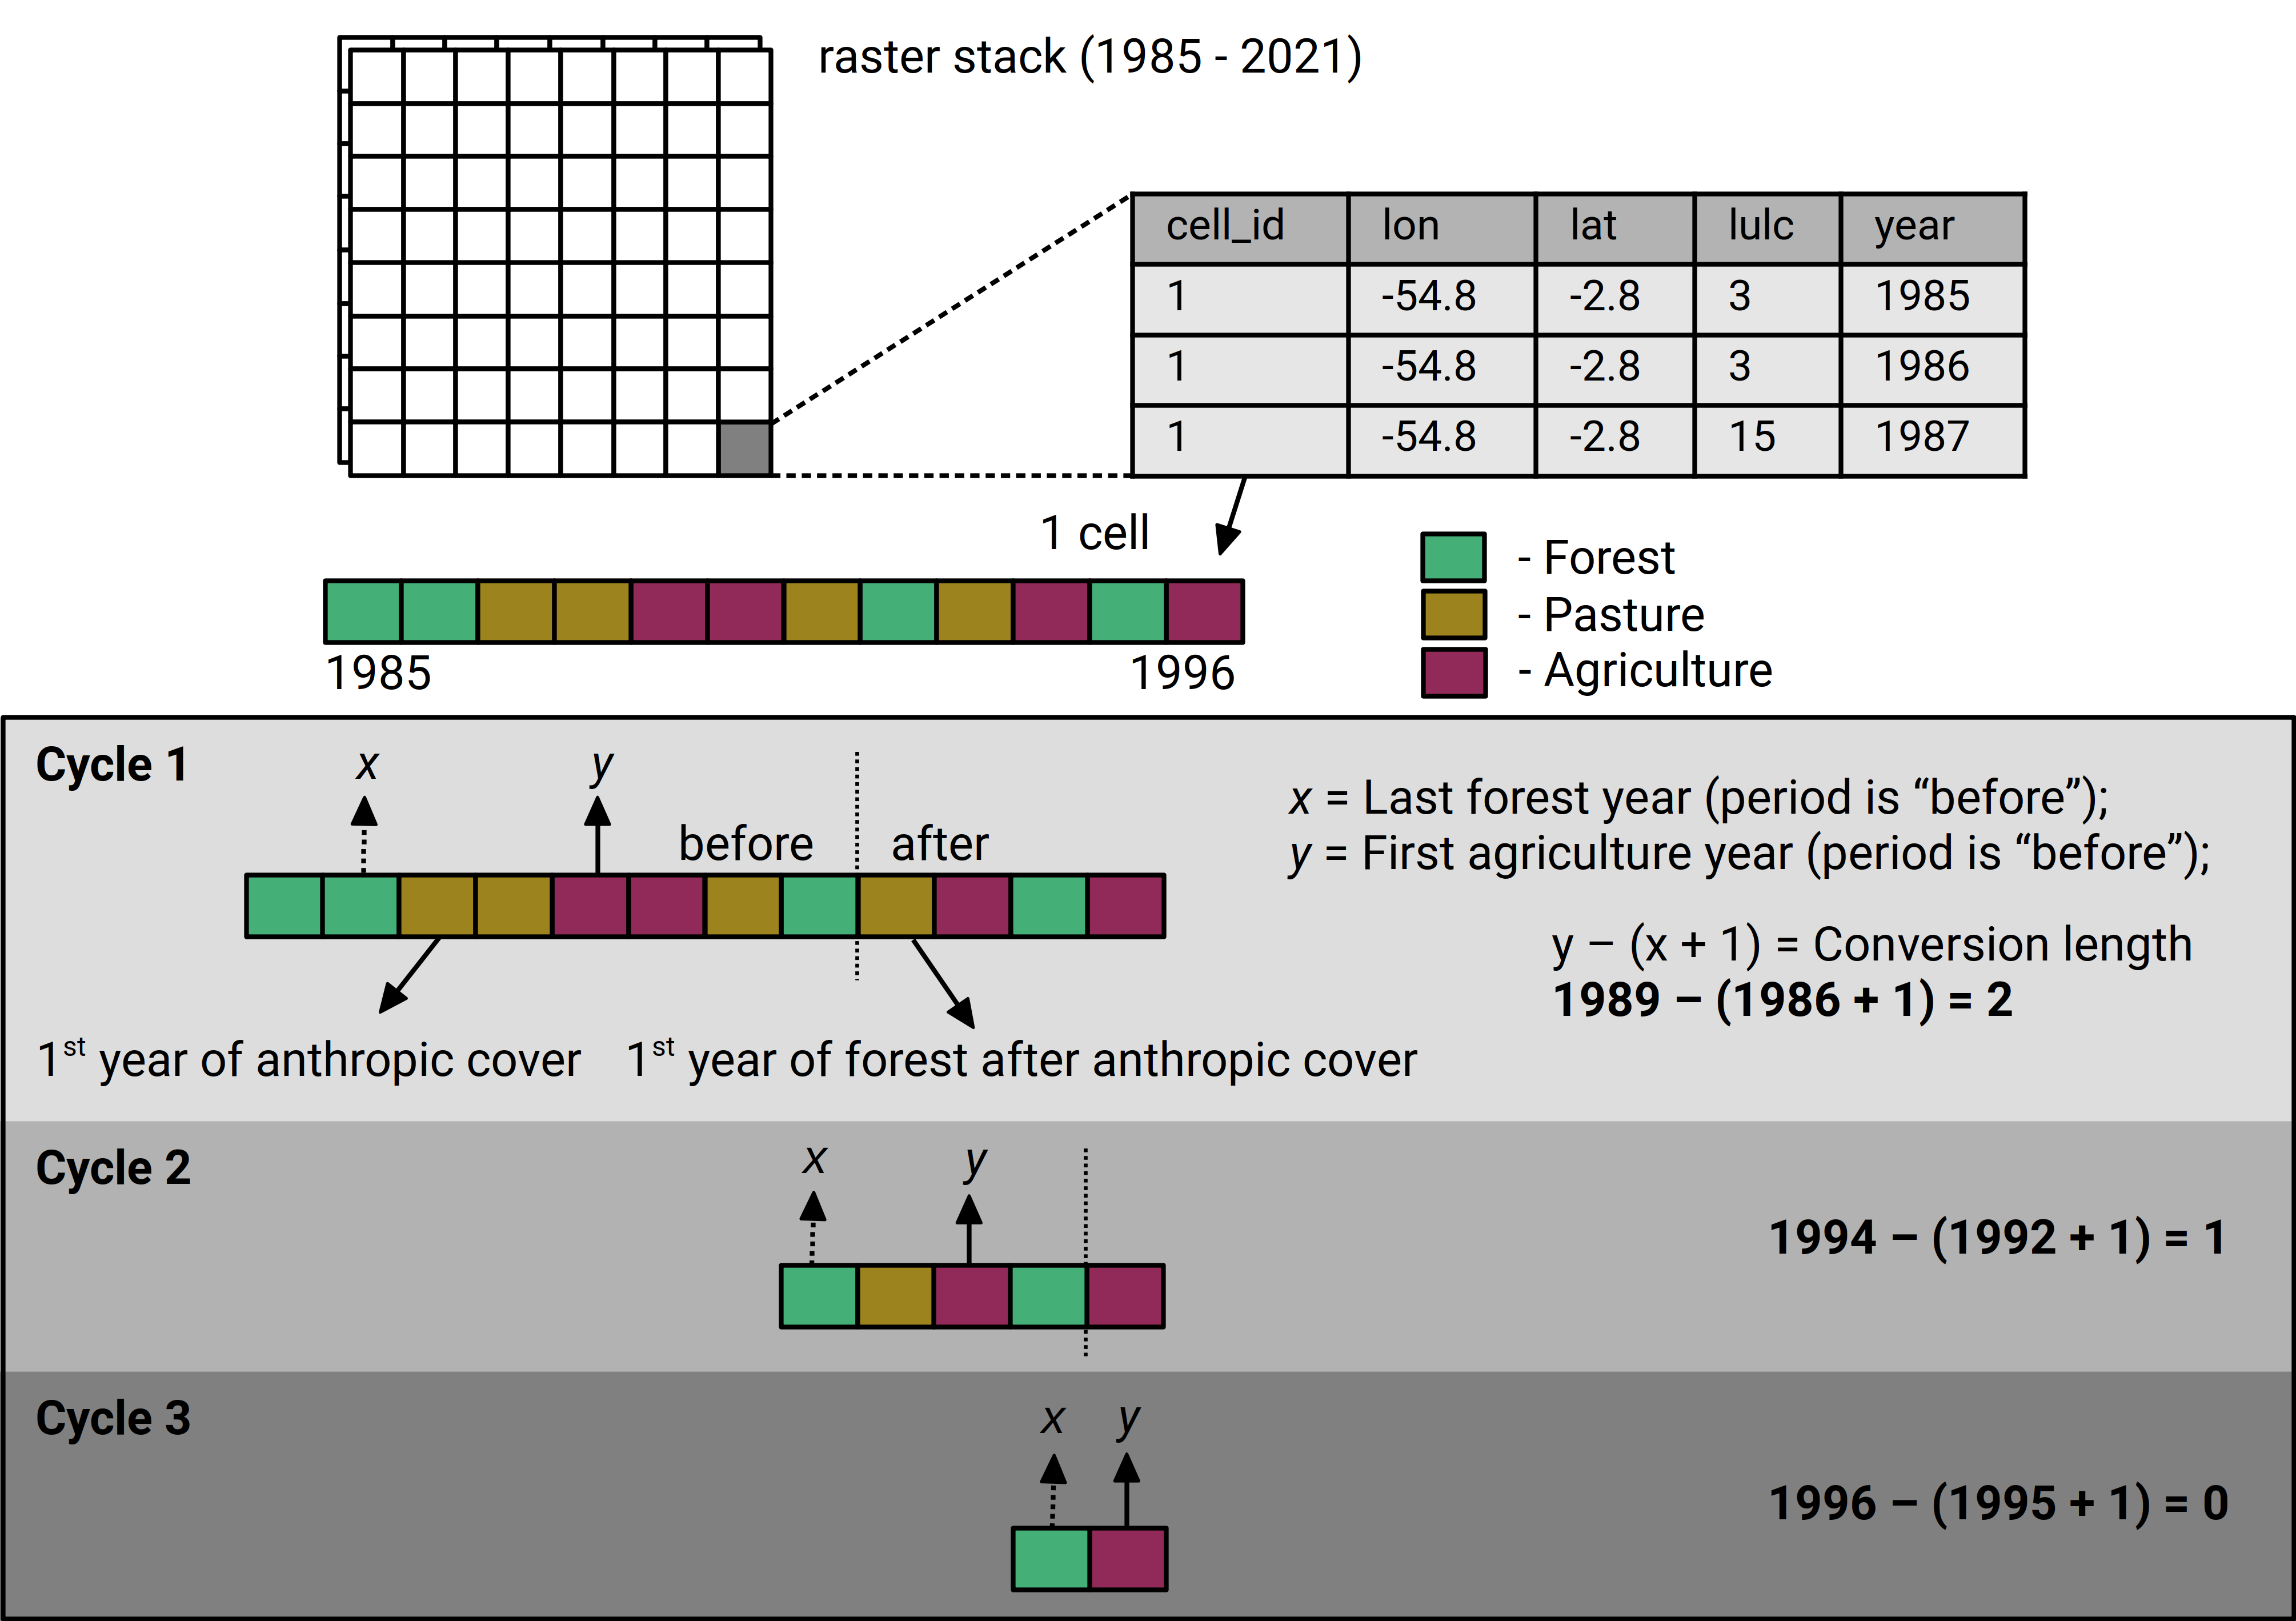
\includegraphics[width=17cm]{figs/change_lenght_routine_scheme} \caption{Representation of the process to calculate the conversion length from forests to agriculture. All values presented are hyphothetical, and serve only as an illustration of the method.}\label{fig:routine-plot}
\end{figure}

The process of calculation of the conversion length (Figure \ref{fig:routine-plot}), can be divided into seven steps of processing:

\begin{enumerate}
\def\labelenumi{\arabic{enumi}.}
\item
  Load raster and extract valid values into a table;
\item
  Calculate the year of first occurrence of any agriculture class (annual and permanent crops) for each pixel;
\item
  Calculate the first year of ``Forest Formation'' LULC class after the year calculated in step 2.
  This step identifies the occurrence of more than one conversion in a given pixel;
\item
  Classify rows as ``before'' or ``after'' the occurrence of the year calculated in step 3.
  This is the identification of periods before and after a return of forest after a first conversion to agriculture;
\item
  Calculate the last year of ``Forest Formation'' within the rows classified as ``before'', and add 1 year to represent the deforestation year;
\item
  Calculate the first year of any agriculture type class within the rows classified as ``before'', for each pixel;
\item
  Calculate the difference between years from items 5 and 6 to get the LULC conversion length in years, for each pixel;
\end{enumerate}

The steps 2 to 7 are performed recursively to identify multiple conversions, in case they are present.
In addition to the conversion length values and the years of the conversion, they are also qualified by the type of agriculture that were established after deforestation, if the conversion occurred from primary or secondary forests, and the number of occurrences of conversions at the pixel.
The LULC classes within the conversion and until 5 years after were also stored.

The conversion results are stored in a data set of tabular files, where data can be queried for further analysis.
After the calculations, data was also converted back to raster format, with the aim to expand the accessibility of the data set.

\subsection{Description of data collection}

After the calculation of conversions, the results are stored in three different types of tables (Figure \ref{fig:tables-plot}), organized in a folder structure and stored as Apache Parquet files.

\begin{figure}[h]
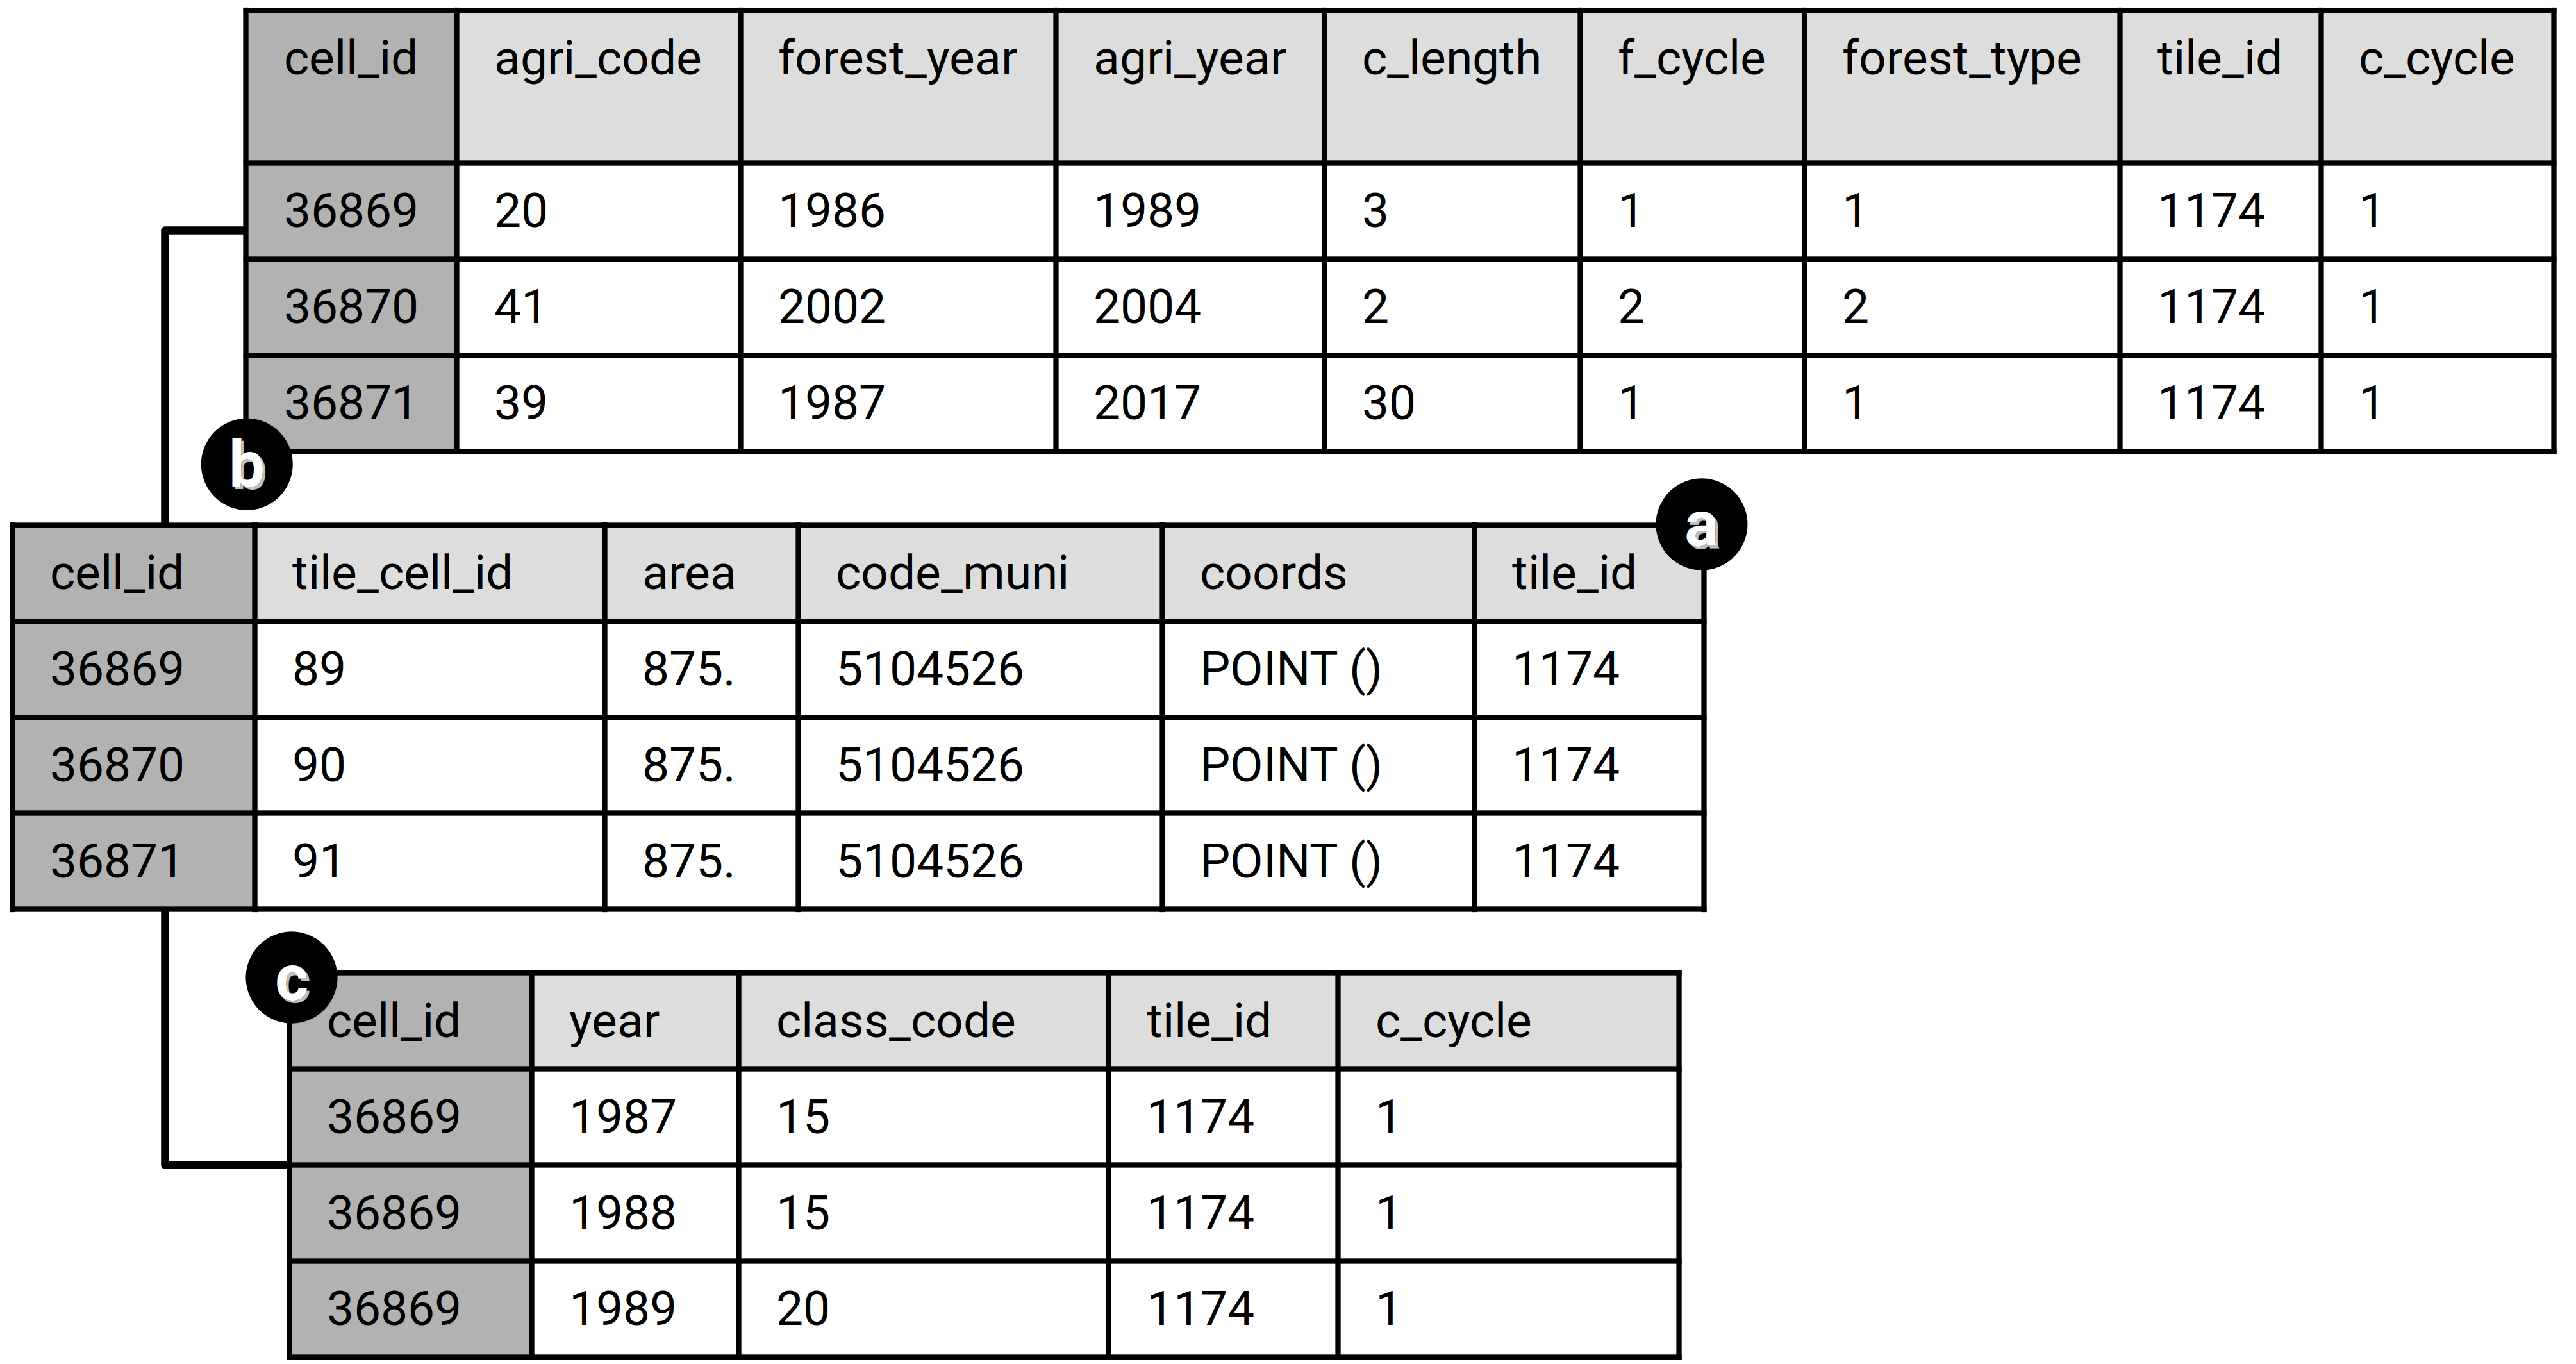
\includegraphics[width=17cm]{figs/tables_scheme} \caption{ Representation of the tables generated by the conversion length calculation. All values presented are hyphothetical, and serve only as an illustration of the method.}\label{fig:tables-plot}
\end{figure}

The first type of table (Figure \ref{fig:tables-plot}.a) contains the spatial information (longitude, latitude and area) of each pixel, its unique identification and the code of the municipality which contains the pixel.
The ``cell\_id'' column contains a unique identification for the whole data, while the ``tile\_cell\_id'' holds a unique value of each pixel for a single tile.
Each tile is also uniquely identified in the column ``tile\_id''.
This table is named ``mask\_cells''.

A second type of tables (Figure \ref{fig:tables-plot}.b) stores conversion length values, the first and last year of the conversion, the resulting agriculture type, and the number of the conversion cycle.
They also contain the unique id of each pixel and tile (related to the table above).
The ``agri\_code'' column holds information about the type of agriculture the was established after deforestation.
The ``forest\_year'' have values that represent the year of deforestation, the ``agri\_year'' is the year when the agriculture establishment happened, and the subtraction between both (the conversion length) is stored in the ``c\_length'' column.
Since it is possible that one pixel contains more than one conversion from forest to agriculture, we stored the number of the conversion in the column ``c\_cycle'' (1 is the first conversion cycle).
However, conversion from forest to other LULC is also possible, so the column ``f\_cycle'' holds information about the number of the conversion from forest to any LULC.
If the forest has suffered any conversion, it starts being considered as a secondary forest, as indicated in the column ``forest\_type''.

The third type of tables (Figure \ref{fig:tables-plot}.c) contains the LULC classes of all years within the conversion, and also the first 5 years after the conversion.
The column ``year'' holds the year of the MapBiomas classification, and the ``class\_code'' variable stores the LULC classification (according to MapBiomas) for the respective year.

The three tables are related to each other and can be used altogether, and are separated by tiles.
Another table containing the metadata of each tile is also created, and holds the spatial characteristics of the tiles.
With this spatial information, it is possible to convert the tabular data back to spatial raster, with identical spatial properties as the original MapBiomas classification data.

The tabular data was organized in a system of folders and sub folders in a hive format partitioning (Figure \ref{fig:dataset-plot}).
This structure allows for easily accessing parts of the data set, and also to filter it without the necessity to read the tables.
In the case of this data set, it is partitioned by the ``tile\_id'' and ``agri\_cycle'' variables.
The data set also has a metadata file with the spatial characteristics of each file, it stores the identification of the tile, the maximum and minimum latitude and longitude, the coordinate reference system, and the number of columns, rows, and cells of each tile.

\begin{figure}[h]
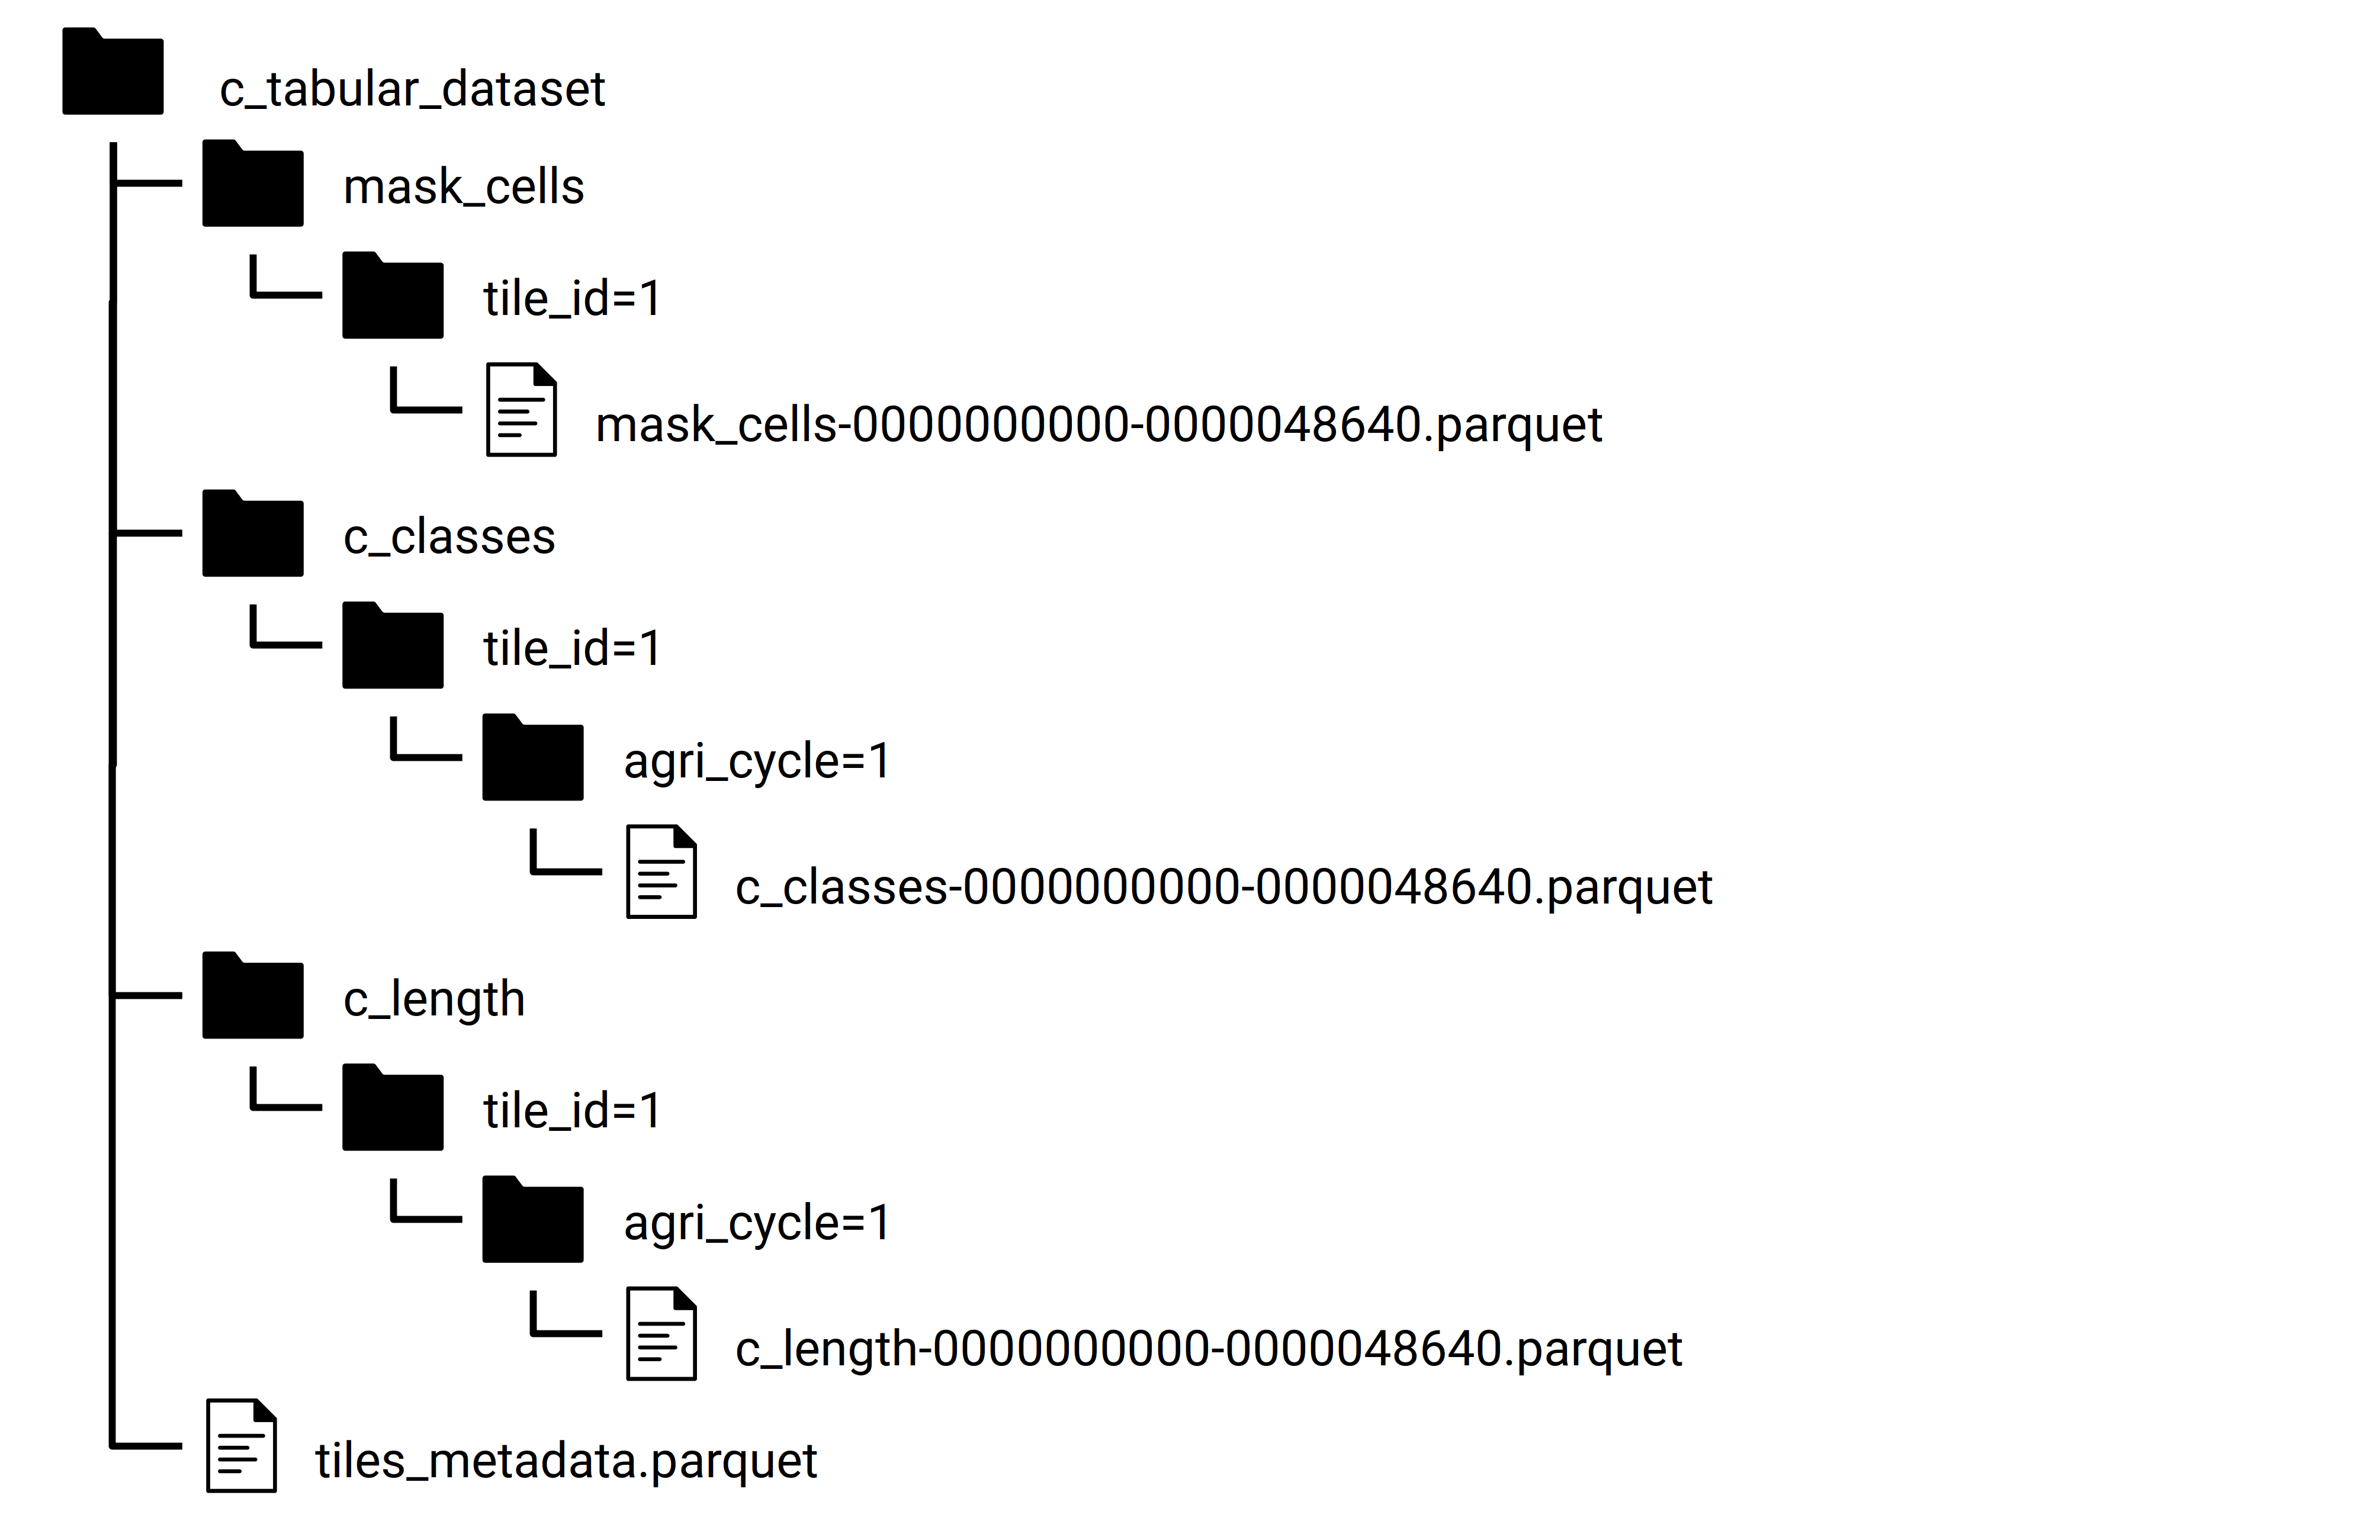
\includegraphics[width=17cm]{figs/dataset_structure} \caption{ Representation of the data set, structured in folders and sub folders.}\label{fig:dataset-plot}
\end{figure}

\subsection{Accuracy assessment}

Accuracy assessment was performed by visual inspection of annual composites of Landsat images from MapBiomas.
We selected 100 random points to be analyzed.
An area of approximately 4 square kilometers around the sample point was used in the visual inspection of satellite images.

The visual inspection used several variables derived from the Landsat historical collection.
The median of Red, Green, Blue, Near Infrared (NIR) and Short Wave Infrared (SWIR1) from dry and wet season were used, and also the annual amplitude of the Normalized Difference Vegetation Index (NDVI).
The process of accuracy assessment was performed in a Shiny app, and was conducted without any consultation to the conversion length results.
In the validation app, we estimated, by visual inspection, the year of deforestation and the year of agricultural establishment.
The observed conversion length was obtained by subtracting both dates.

To evaluate the accuracy, we calculated the Mean Absolute Error (MAE), the Bias (BIAS), and the Percent Bias (PBIAS).
We also analyzed the results by plotting the errors as frequency bars, and scatter plots between observed and estimated values.
After the completion of the analysis of the 100 sample points, we also conducted a qualitative assessment, where we compared our results with satellite images composites.

\section{Results and discussion}

The conversion calculations show that in the Brazilian Amazon biome, 64874 square kilometers of forests were converted to agriculture between 1985 and 2021.
The length of the conversions can go from 0 to 35 years, in which conversions closer to 0 years are considered as fast conversions, and conversions closer to 35 years are considered as slow conversions.
Transitions of 0 years are considered ``direct'' conversions, where there was no presence of pasture before the establishment of agriculture.
Our estimations show that around 9.2\% of the conversions were ``direct''.

Our conversions calculations found pixels that presented up to six conversions from forest to agriculture since 1985, as these numbers are unlikely to happen (they are distributed as sparse pixels, and do not show patterns of real conversions, being common at borders), we proceeded the results analysis only in the first conversions found in each of these pixels.

Although we named the year of change from forest to anthropic land uses as deforestation, we acknowledge that it is not a direct measurement of deforestation (such as PRODES), however it represents a proxy to deforestation.

\subsection{Transition patterns}

Transitions from forest to agriculture can be found in almost every region in the Amazon, but is mostly concentrated in clusters, specially in the south and east of the biome, in the states of Mato Grosso, Pará and Maranhão (Figure \ref{fig:map-plot}).

\begin{figure}[h]
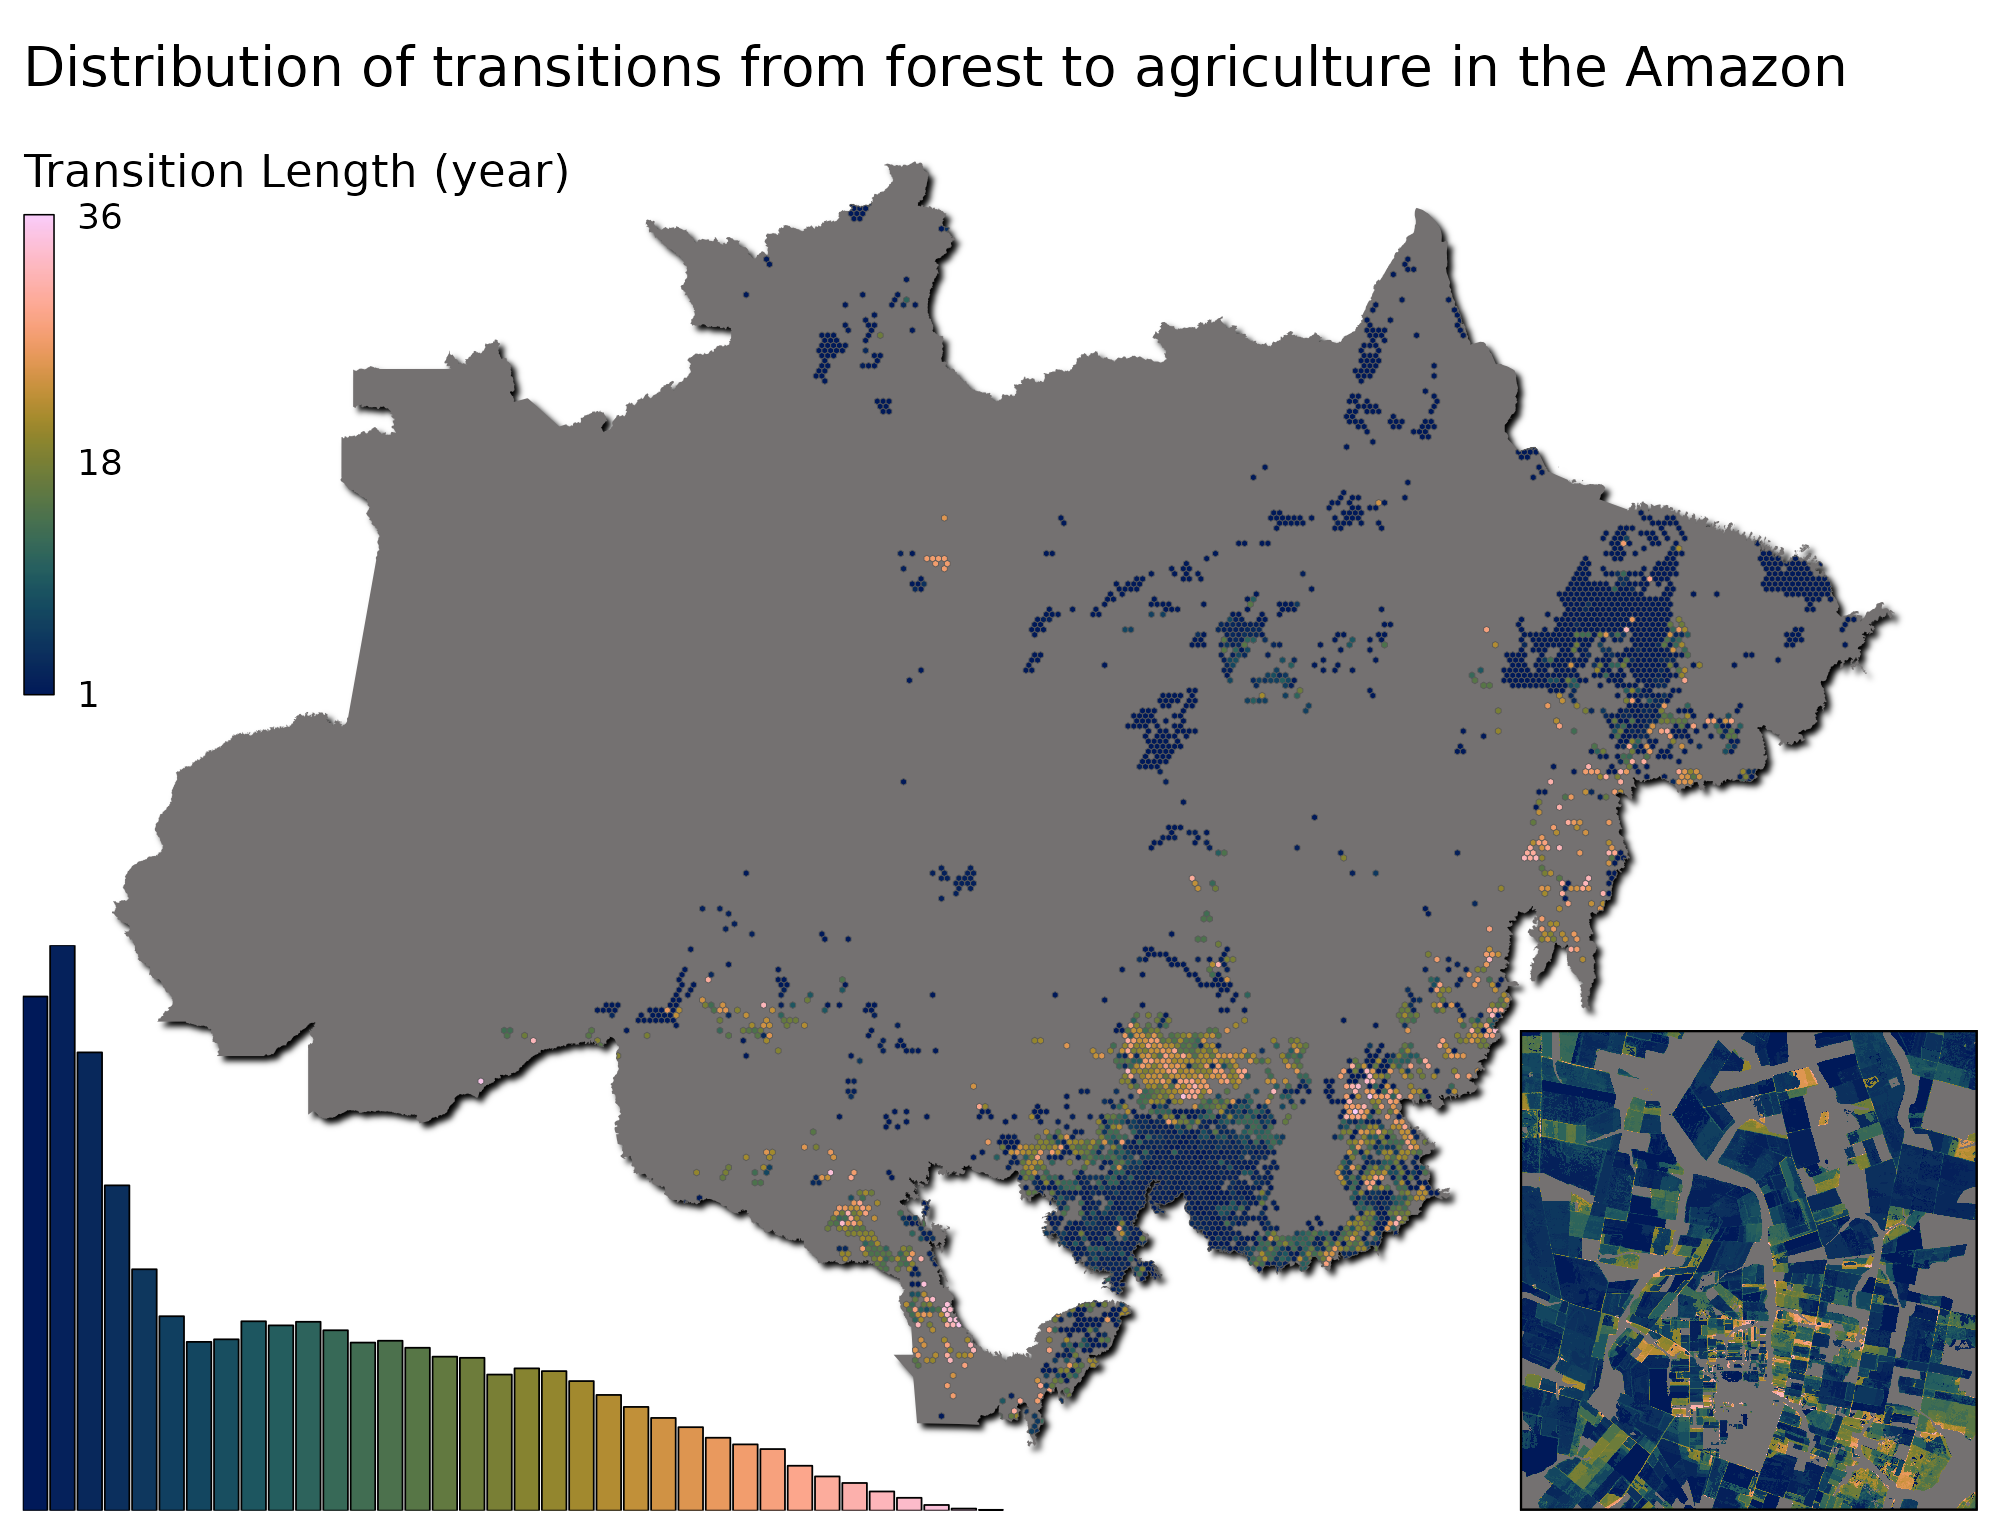
\includegraphics[width=17cm]{figs/map} \caption{Map of distribution of conversions from forest to agriculture in the Brazilian Amazon biome. The hexagonal cells represent the most common conversion length, and do not reflect the amount of area of conversions inside a cell. Transitions are concentrated in the south (Mato Grosso state), and in the east (Pará and Maranhão states). The conversion length ranges from 0 (dark blue) to 35 years (light pink), and clusters of fast conversions (conversions closer to 0 year) can be discerned from clusters of slow conversions (conversions closer to 35 years). The histogram located in the bottom left shows that fast conversions are more common than slower conversions. The zoomed map in the bottom right shows the results in finer resolution, where it is possible to observe different conversion lengths between properties. The red square shows the extent of the zoomed map.}\label{fig:map-plot}
\end{figure}

Well defined clusters can be observed in the map created with aggregated conversion length data (Figure \ref{fig:map-plot}).
Slow conversion areas tend to concentrate in specific regions of the biome, while fast conversions seem to have a wider distribution, but also tend to form spatial clusters.
However, this pattern does not hold completely when observing the data at its original scale (Figure \ref{fig:map-plot}), where areas with different conversion lengths are mixed between each other.
When observing at the original scale, we could not spot any well defined pattern or direction of the occurrence of faster to slower conversions (Figure \ref{fig:map-plot}).
Other studies investigating patterns of conversions in the Amazon also found the formation of clusters of patterns, although there is a big heterogeneity at larger scales \citep{MullerHansen2017}.

The data can be analyzed year by year, and also be separated by primary and secondary forests being converted to agriculture (Figure \ref{fig:transbar-plot}).

\begin{figure}[h]
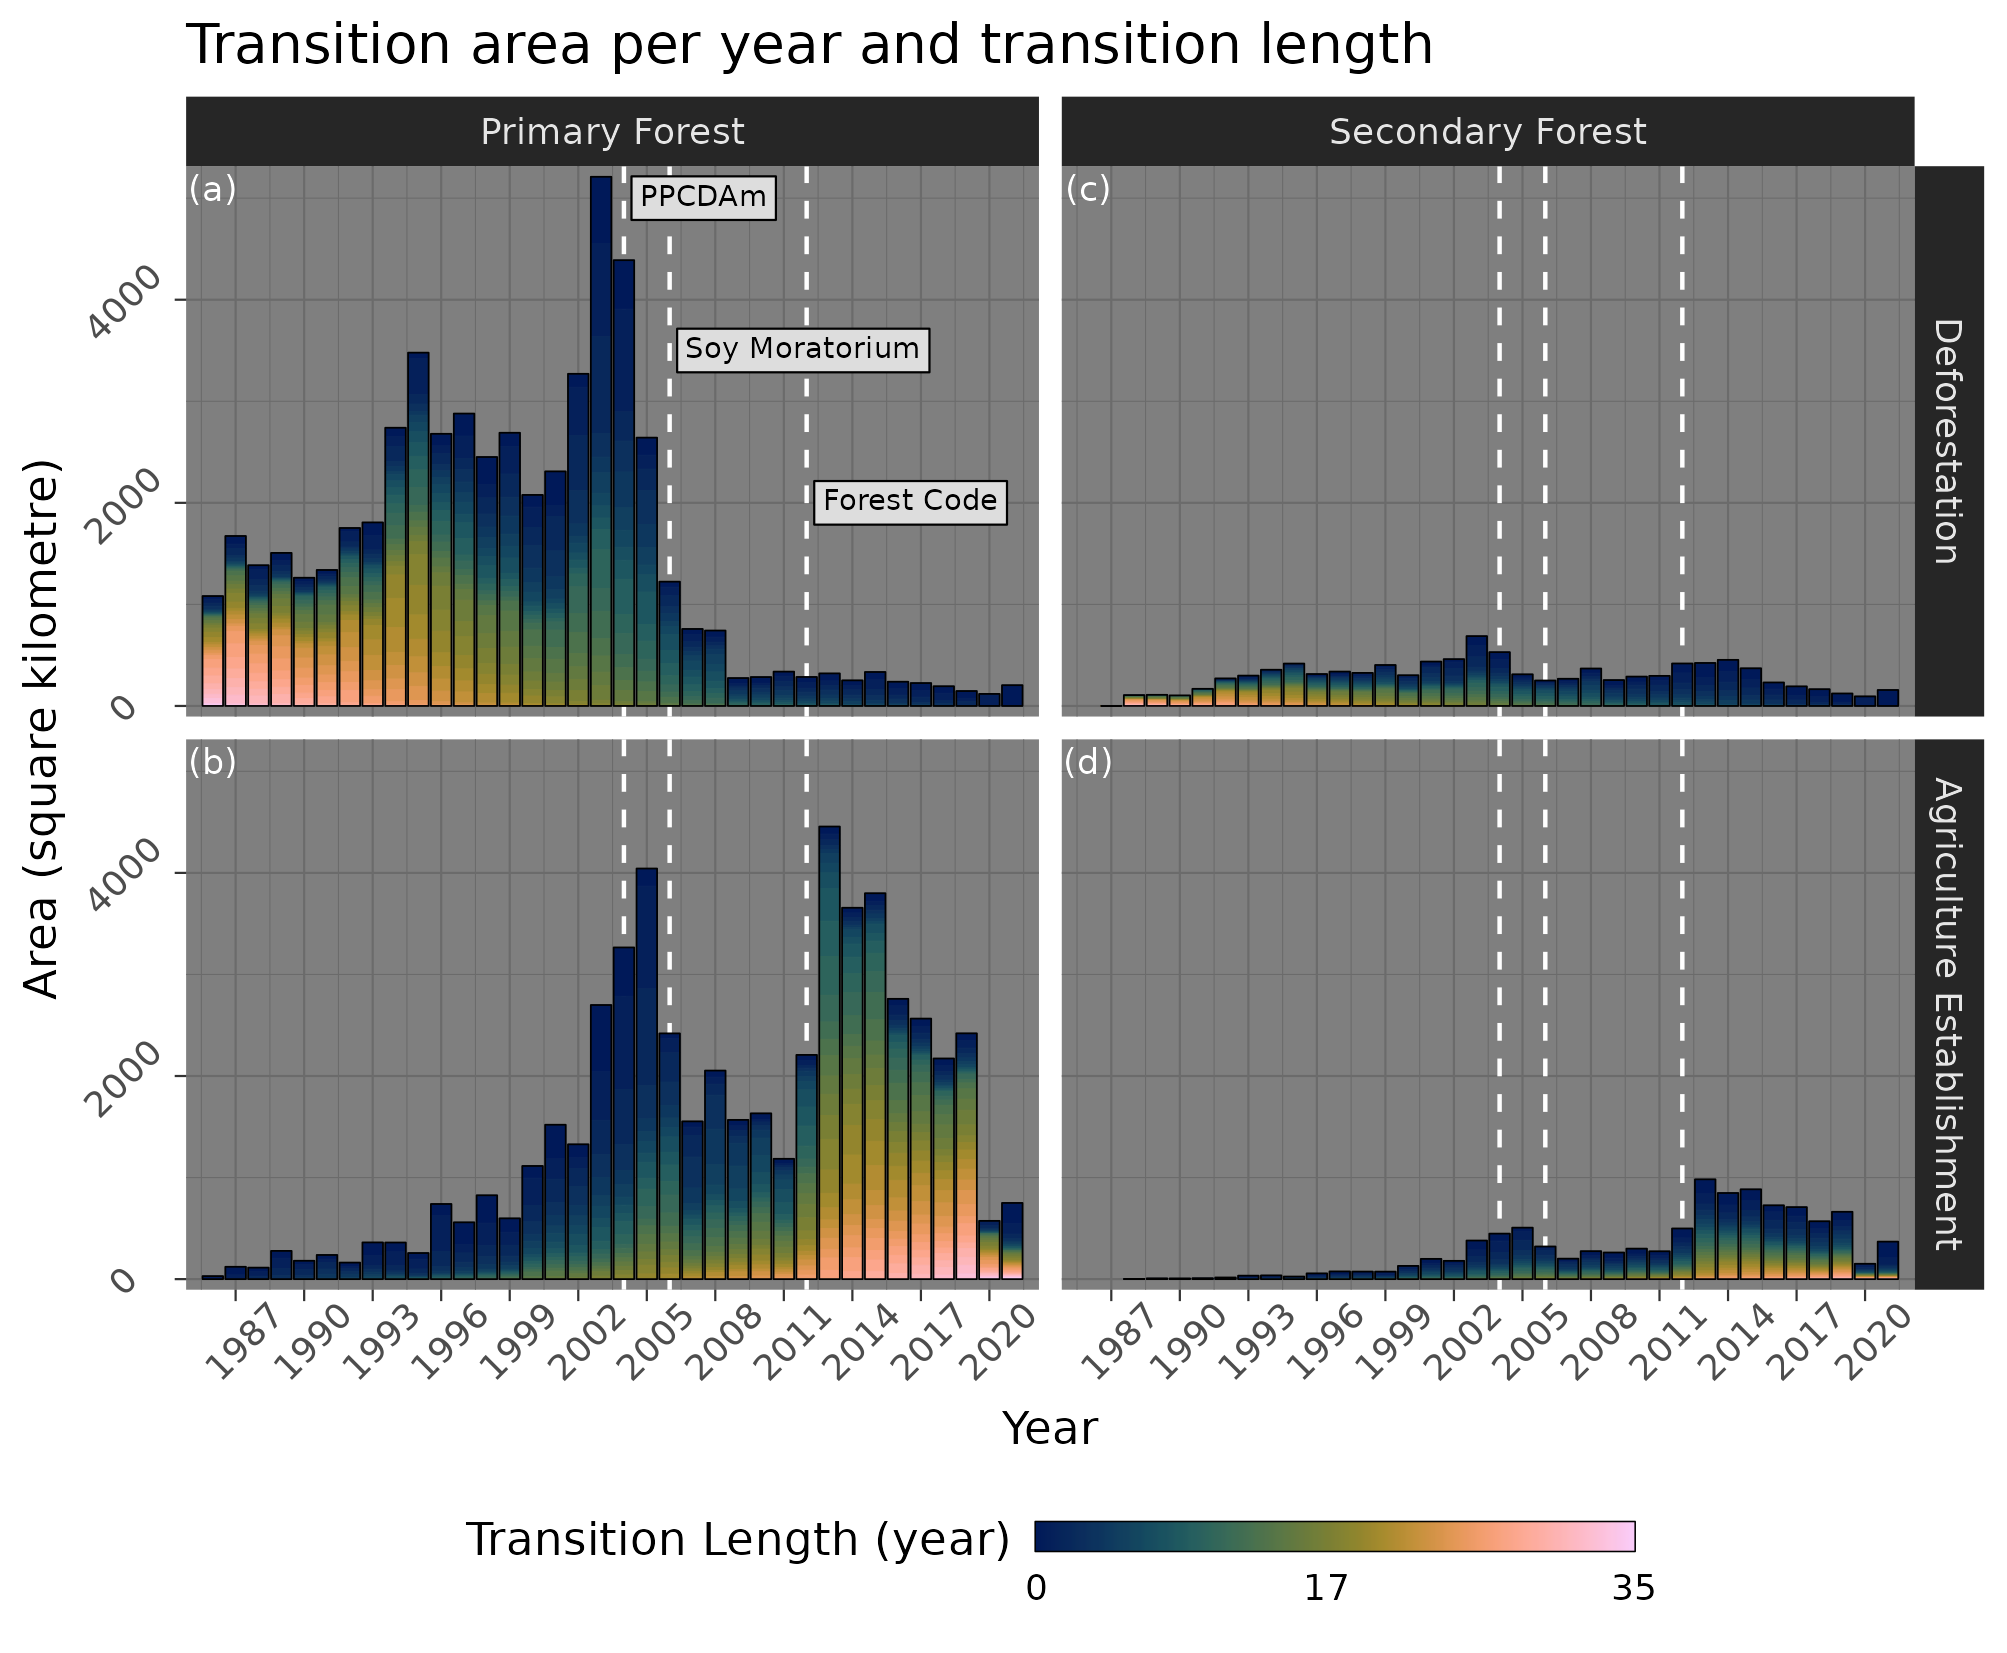
\includegraphics[width=17cm]{figs/trans_length_cols} \caption{Transition area from forest to agriculture, per year and conversion length. The bars represent the total amount of area at some state of the conversion for each year. The color gradient in each bar represent the conversion length related to a deforestation or an agriculture establishment event. Blue tones represents fast conversions (closer to 0 years), pink tones represent slow conversions (closer to 35 years). Transition events were separated by deforestation of primary forests (a) and secondary forests (c), and the subsequent agriculture establishment of primary forests (b) and secondary forests (d).}\label{fig:transbar-plot}
\end{figure}

The deforestation area of primary forests increased largely from 1986 to 2003, which was followed by a steep decrease until 2009, when the deforested areas reached a stable rate (Figure \ref{fig:transbar-plot}.a).
From 1985 to 1995, most deforested areas suffered a slow conversion, mostly were higher than 10 years (76 \%).
After this period, fast conversions started to become more common (Figure \ref{fig:transbar-plot}.a), specially from 2002 to 2004, where 70 \% of the transitions were faster than 10 years.
Our results show that in 2003 (the peak of deforestation), 12.7\% of the conversions were a direct conversion from forest to agriculture.
Previous studies estimated a proportion of 23 \% in the Mato Grosso state, for the same year \citep{Morton2006}.
If we include fast conversions (from 0 to 2 years) from our results, the proportion jumps to 48.1 \% of all conversions in 2003.

Agricultural establishment over areas of primary forests peaked in 2005 and 2013 (Figure \ref{fig:transbar-plot}.b).
Despite similar agricultural establishment areas in both years, their conversion lengths differ greatly (Figure \ref{fig:transbar-plot}.b), in 2005 most of the conversions were faster than 10 years (78 \%), while in 2013 the majority of conversions were slower than 10 years (66 \%).
In 2010, it was observed a shift in the conversion length from forest until the establishment of agricultural areas.
From this year onward, 68 \% of the conversions happened in areas deforested at least 10 years before (Figure \ref{fig:transbar-plot}.b).
Even after the decrease of deforestation after 2002, areas under agriculture expanded over lands where deforestation happened before 2002 (mostly over pastureland).
However, after 2019, a sudden drop of agriculture establishment rate happened (Figure \ref{fig:transbar-plot}.b).
This behavior could be related to economic causes or even the scarcity of suitable areas for agricultural expansion, which seems unlikely, since the last years have been marked by an increase of deforestation rates and the advance of pastureland over the forest.

The causes of deforestation and agricultural establishment in the Brazilian Amazon are complex and diverse.
Political context, public policies, market prices and law enforcement can influence how these processes evolve over time.
The end of the 1980s and the 1990s were marked by the development of policies for protection of the environment, with the creation of the National Environmental Policy, the establishment of the Brazilian Institute of Environment and Natural Resources (IBAMA), and the Ministry of Environment \citep{Banerjee2009}.
However, this new policy environment was not immediately translated into a significant deforestation decrease in the Amazon, which remained at high levels until the beginning of 2000s.
Our results show that deforestation in this period (1986 - 2000) was mainly followed by pasture, which remained for a long time before being converted to agriculture (Figure \ref{fig:transbar-plot}.a).

Apart from protectionist policies created in the 1990s, development programs kept pressuring forests in the Amazon.
In the late 1990s, the development policies ``Brasil em Ação'' and ``Avança Brasil'' (1995 - 2003) accelerated the national infrastructure expansion, including in the Amazon \citep{Carvalho2002}.
This is a period when the deforestation areas reached the highest values in the time series (Figure \ref{fig:transbar-plot}.a), and also a peak in the establishment of agriculture in the Amazon biome, predominantly with fast conversions (Figure \ref{fig:transbar-plot}.b).

In 2004, the Brazilian Government launched the Action Plan for the Prevention and Control of Deforestation in the Legal Amazon (PPCDAm), which was composed of many initiatives to curb deforestation \citep{West2021}.
The PPCDAm was considered as a successful policy to slow deforestation rates in Brazil, with international recognition.
Our calculations from MapBiomas data reinforces the correlation of the PPCDAm with the reduction of deforestation after 2004 (Figure \ref{fig:transbar-plot}.a), and reduction of the agriculture establishment after 2005 (Figure \ref{fig:transbar-plot}.b).

In 2006, the Brazilian Association of Vegetable Oil Industries (BIOVE) and the National Association of Cereal Exporters (ANEC) committed to avoid commercialization of soybean grains harvested from areas deforested after 2008, known as the soy moratorium.
The soy moratorium is considered to have contributed to the decline of the deforestation directly related to soybean expansion \citep{Paim2021, Amaral2021, Heilmayr2020, Kastens2017}. Our estimates of conversions show a decrease of deforested areas after 2008, where it reached minimal values (Figure \ref{fig:transbar-plot}.a). After 2006, agriculture establishment over deforested primary forests suffered a decrease, which stayed relatively stable until 2012, where a steep increase occurred, however, the new areas being occupied by agriculture were mainly over areas that were cleared before 2008 (Figure \ref{fig:transbar-plot}.b). The period between 2006 and 2010 is also considered as a turnover point, known as the decoupling of deforestation and soybean production, where the total production was not as dependent on agriculture expansion as before \citep{Macedo2012}. Therefore, the observed increase of agricultural establishment after 2012 shows that agriculture expansion did not halt after the soy moratorium nor after periods of high soybean productivity. Producers started to expand over areas cleared many years ago, which may still have indirect impacts on deforestation increase over distant areas \citep{Arima2011, Gollnow2018}. However, this indirect effect is not always clearly observed when analyzing the Amazon biome as a whole, our data shows that periods of fast agriculture expansion occurred at the same time with minimal deforestation values, according to PRODES estimates \citep{Assis2019}. Expansion of agricultural areas also occurred over cleared areas of secondary forests in 2012, but with an important amount of fast conversions (Figure \ref{fig:transbar-plot}.d). The causes of the increase of agricultural establishment areas can be numerous, and one main driver was the approval of a new Forest Code, in 2012, which is considered to have undermined the environmental protection of forests \citep{Kroger2017, Pereira2019}, since it opened the possibility of amnesty for illegally deforested areas \citep{Schielein2018, Santanna2021, Filho2014}, and the possible reduction of legal reserve area \citep{Freitas2018}.

Even though it is possible to analyze the results in the Amazon as a whole, the conversion length patterns across years can change significantly between different states (Figure \ref{fig:transridge-plot}).

\begin{figure}[h]
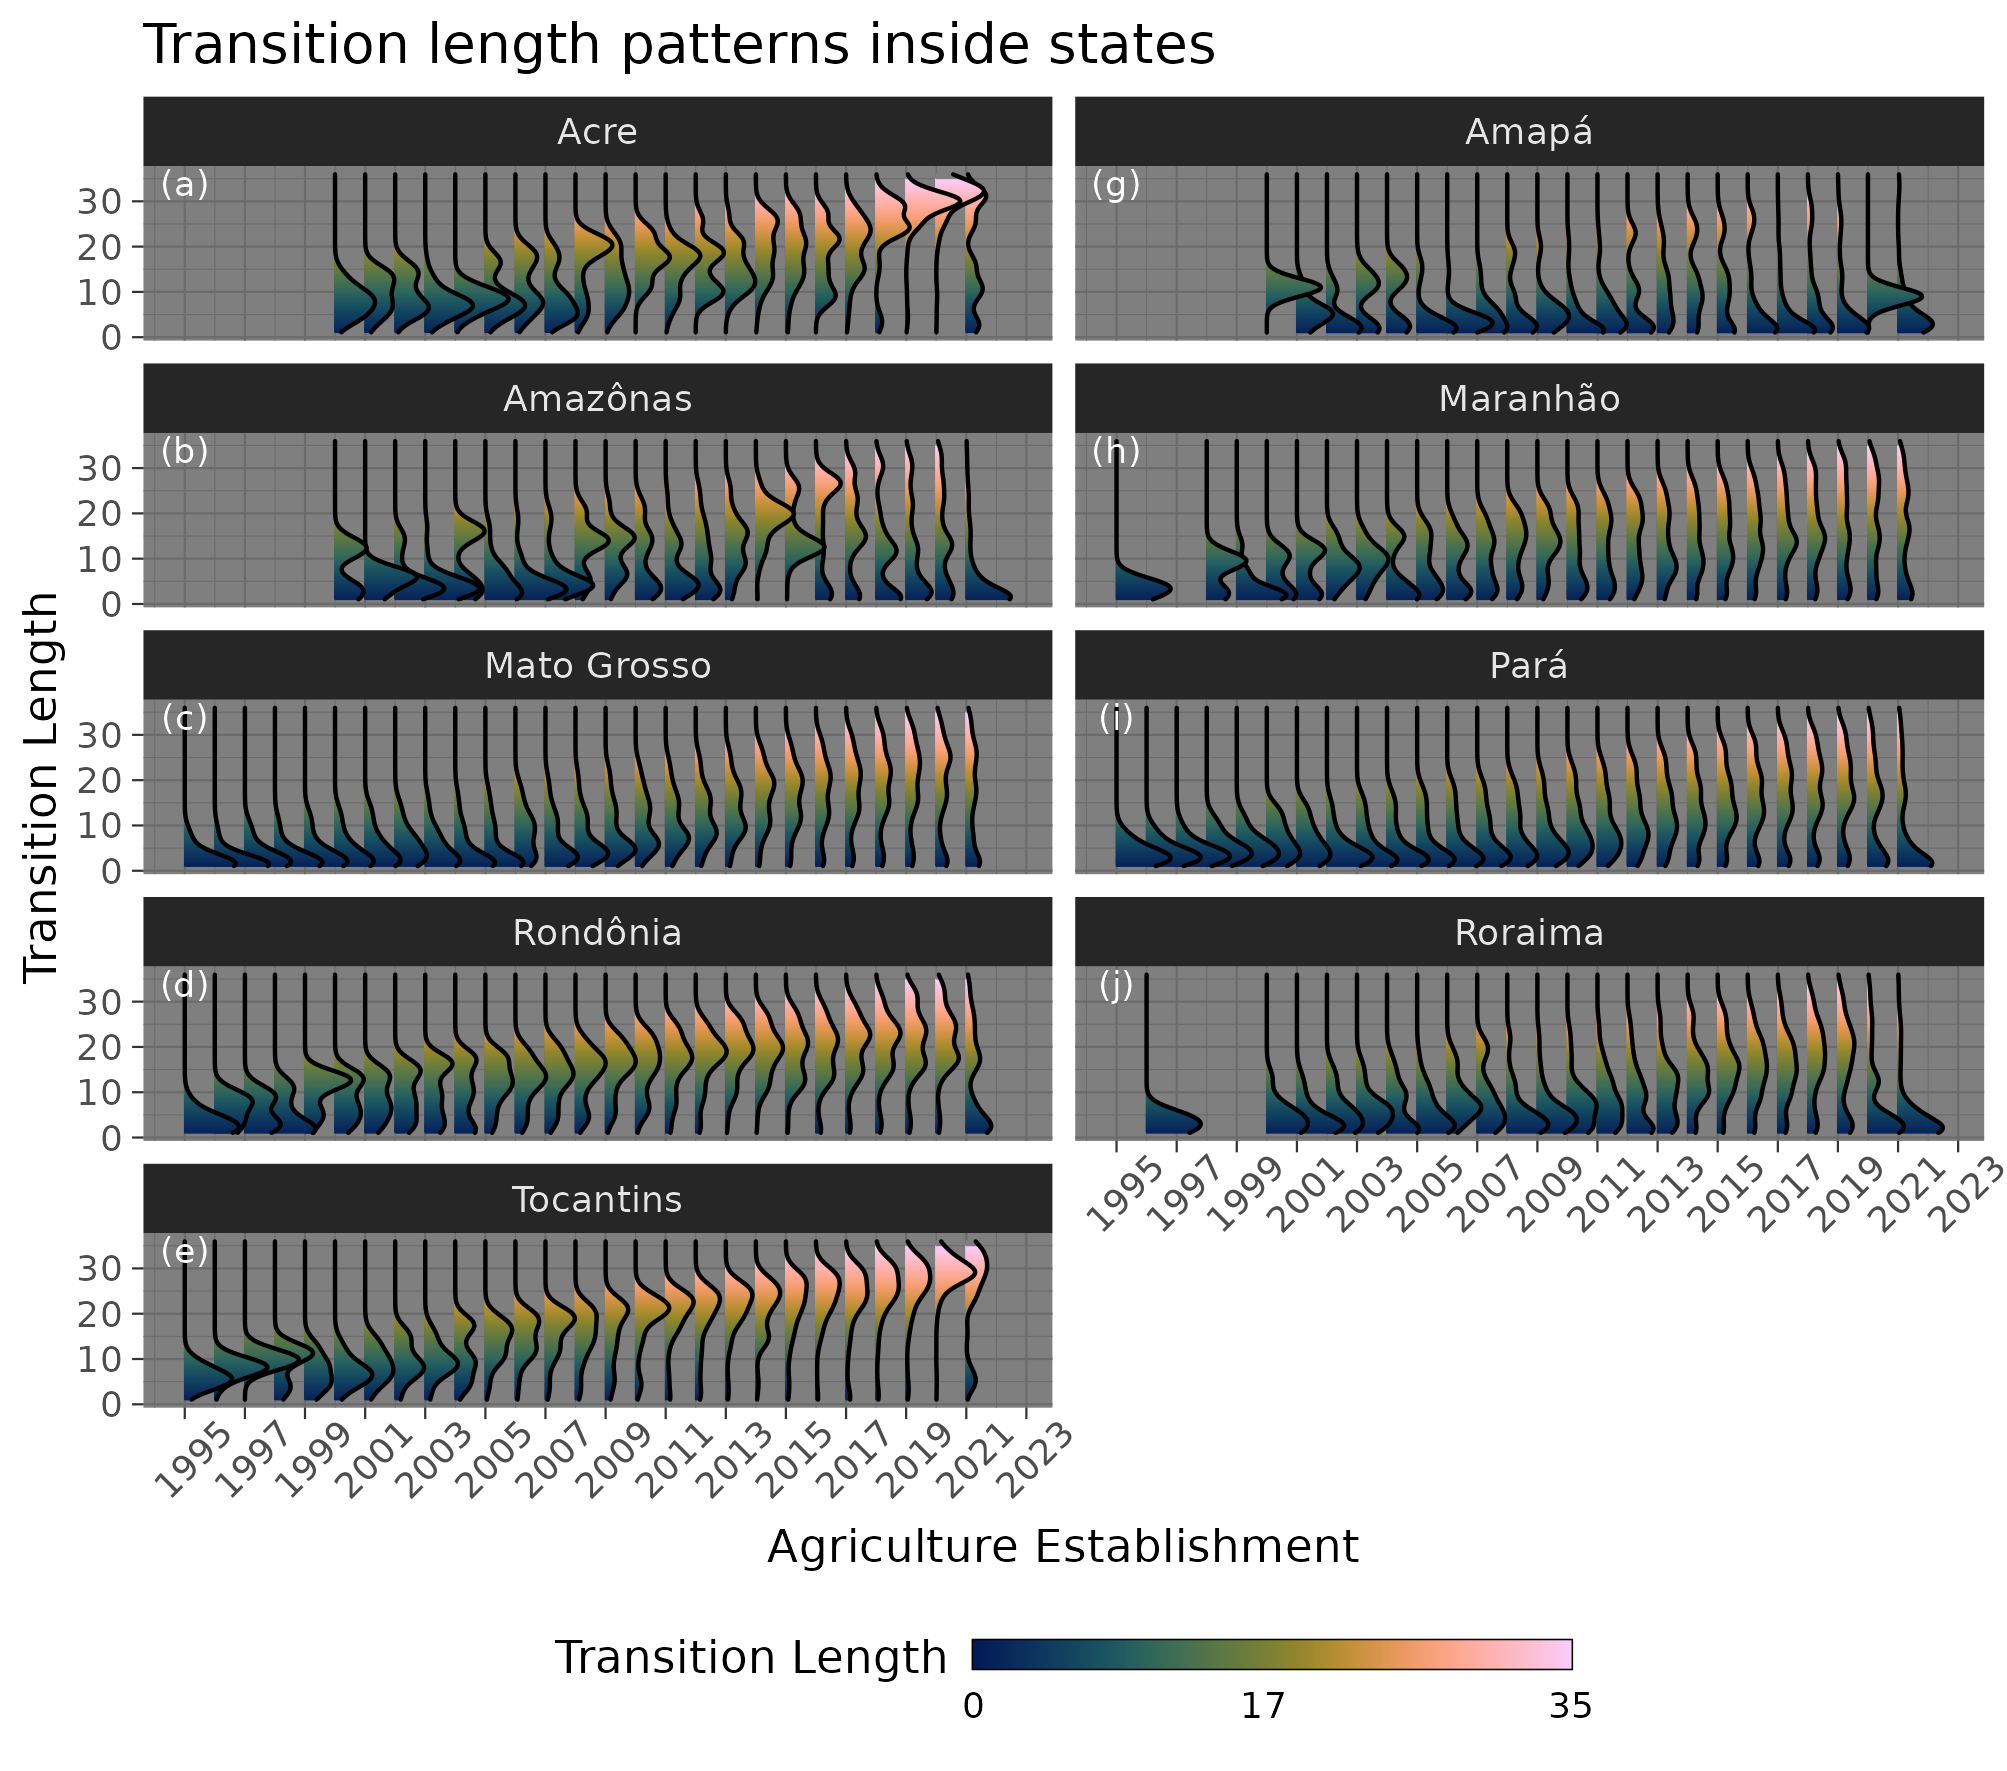
\includegraphics[width=17cm]{figs/trans_ridge} \caption{Transition length patterns inside states in the Amazon biome. Each year has a density estimate of the conversion lengths, represented as colored curves. The peak of the curves represents conversion length values with more frequency in one year of one state. Blue tones represent fast conversions (conversions closer to 0 years), pink tones represent slow conversions (conversions closer to 35 years).}\label{fig:transridge-plot}
\end{figure}

The state of Amapá presented fast conversions along all the time series, without any significant period of slow conversion.
In contrast, conversions in Acre were majorly slow, in which only 2021 showed faster conversions.
There are two states where the pattern of conversion length are alike, Mato Grosso (MT) and Pará (PA).
Both states underwent fast conversions from 1995 to 2005, and after this period slow conversions became predominant until the end of the time series.
Rondônia (RO) and Tocantins (TO) presented a similar pattern of MT and PA, in which conversions decelerated , but for RO and TO since the beginning of 2000s, earlier than MA and PA.

The great majority of conversions are from forests to soybean and ``Other Temporary Crops'', which represents 95\% of the conversions in the Amazon biome (14\% of Soybean and 81\% of ``Other Temporary Crops'').
When analyzing what happened after 5 years since the conversion, soybean areas persistence rate was at 79\% (i.e., areas that remained as soybean), 14\% was converted to ``Other Temporary Crops'' and 7\% was converted to pasture.
``Other Temporary Crops'' are less persistent.
Hence, 27\% of these areas remain in the same class, 56\% were converted to soybean, and 15\% to pasture.
Conversions from soybean and ``Other Temporary Uses'' to other LULC classes (apart from the already cited) are negligible.
Sugar cane, cotton and perennial crops also appear, but in a negligible proportion.

\subsection{Validation}

From the 100 random sample points used in the results validation, 1 point (sample 21) was not considered as a conversion from our estimations, however, the visual inspection pointed to a likely event of conversion from forest to agriculture.
Also, there were 6 points (sample 6, 7, 55, 56, 78, 97) which the visual inspection did not find a conversion from forest to pasture, although our estimations pointed as conversions.
Therefore, 7\% of the sample were completely misclassified by our estimates, and the rest of the accuracy assessment was performed over the remaining 93 sample points.

When analyzing the errors from the conversion length estimates, we observed that the year of deforestation shows the least amount of errors (Figure \ref{fig:errorbar-plot}).
The MAE of the deforestation year is 1.42 years, and the error shows a bias towards underestimation.
The year of the agriculture establishment and the conversion length estimates showed larger errors when compared with visual inspection.

\begin{figure}[h]
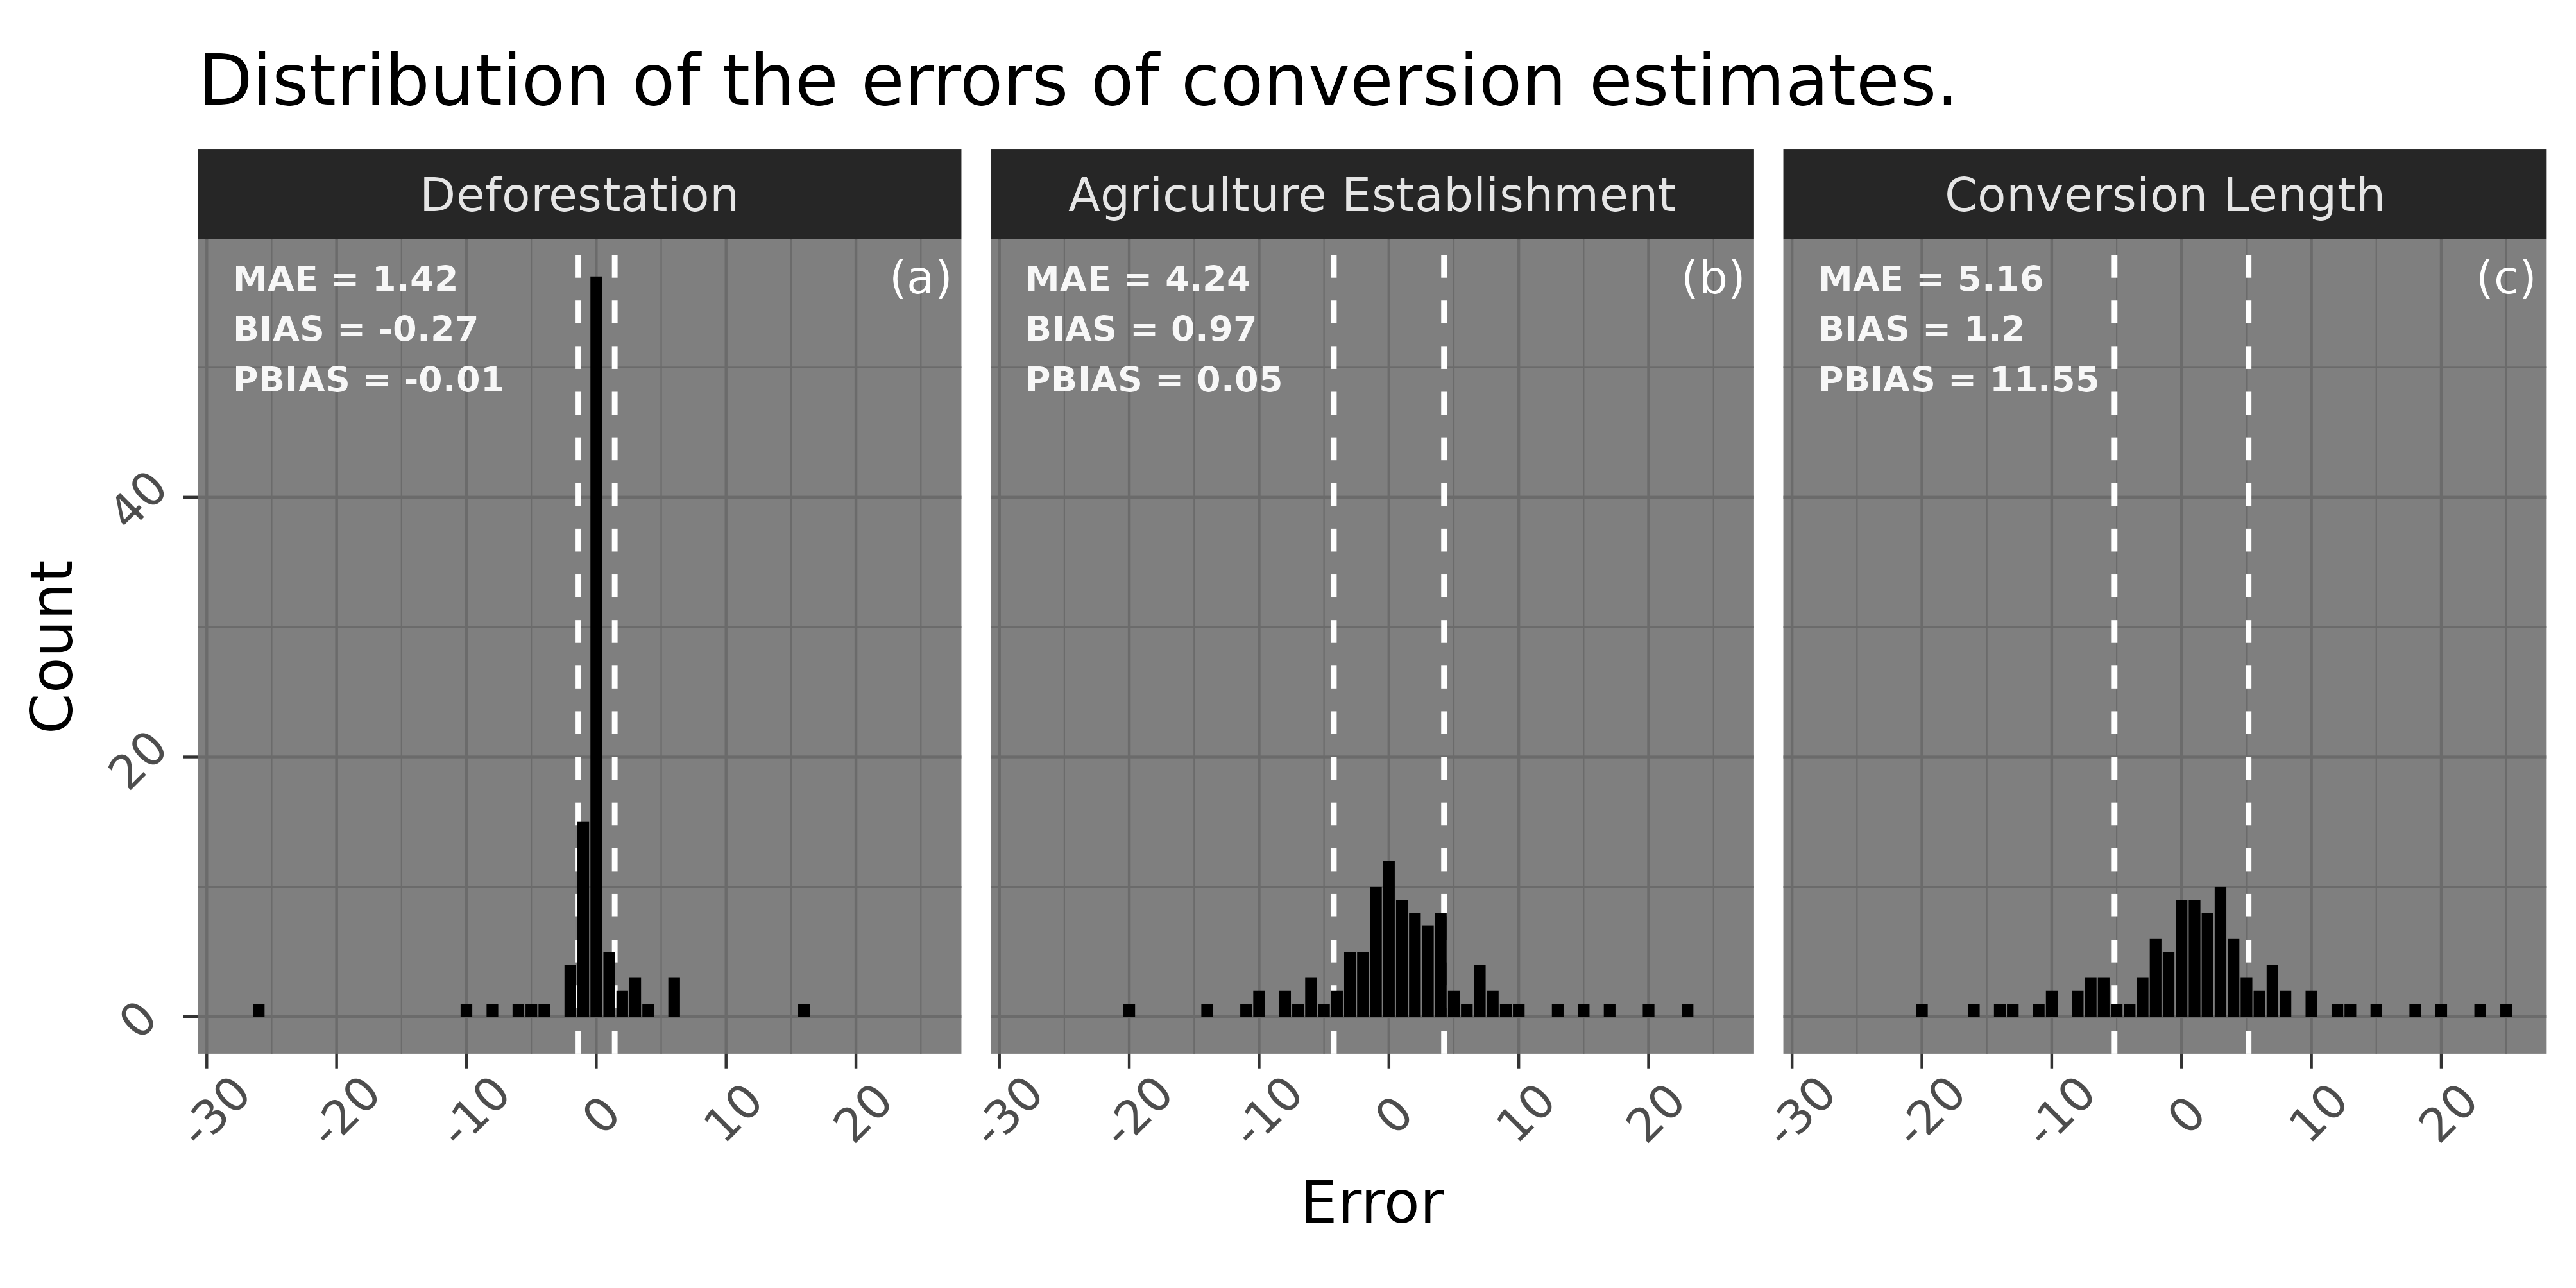
\includegraphics[width=17cm]{figs/error_bars} \caption{Bar with the count of error values (difference between observed and estimated values). Positive values indicate underestimation of the variable (estimations were lower than observations), negative values indicate overestimation (estimations higher than observations). Error metrics (Mean Absolute Error, Bias and Percent Bias) are displayed in the top right position of each box. The white dashed lines represent the MAE values of each variable.}\label{fig:errorbar-plot}
\end{figure}

The dispersion of observed and estimated values shows no clear pattern of errors (Figure \ref{fig:errorscatter-plot}).
Transition length values are more concentrated in smaller values, which also shows higher errors (Figure \ref{fig:errorscatter-plot}.c).
However, this is expected since faster conversions are more common (Figure \ref{fig:map-plot}).

\begin{figure}[h]
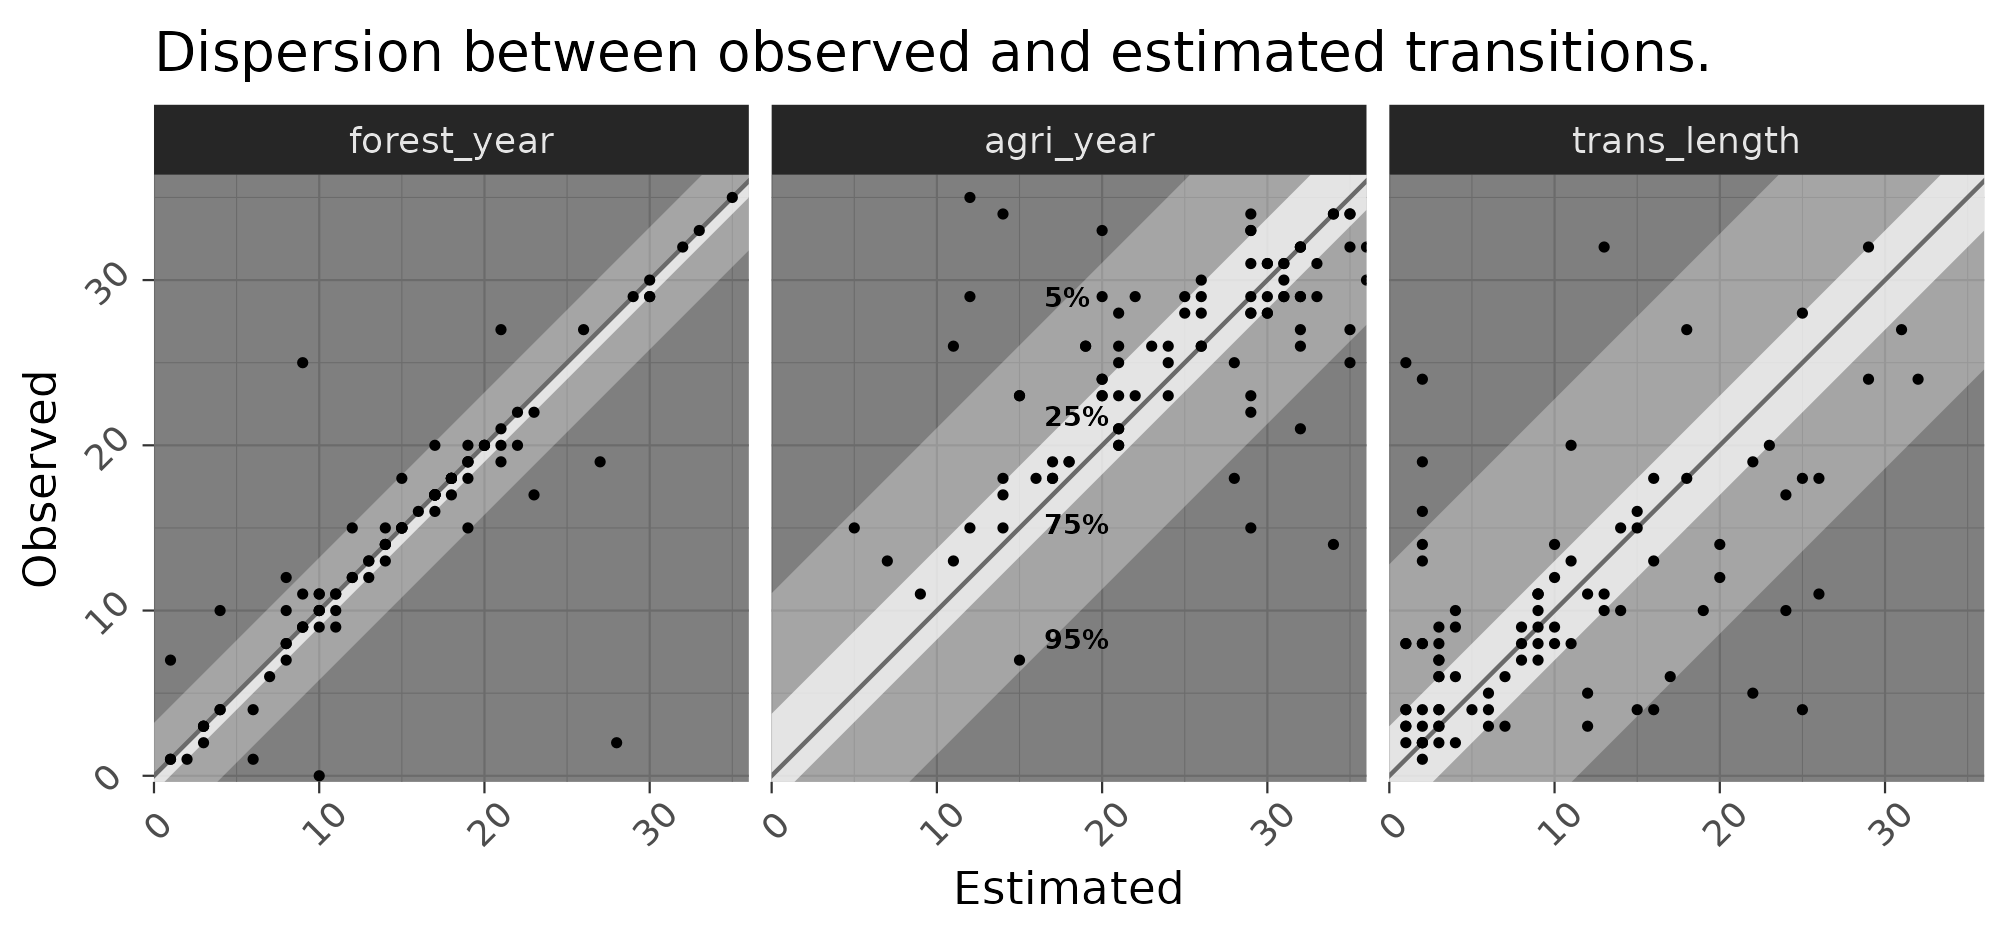
\includegraphics[width=17cm]{figs/error_scatter} \caption{Scatter plot between paired values of estimated and observed Deforestation and Agriculture Establishment years, and their respective Transition Length. The gray line represents values where there would be no errors of the estimated values in comparison with the observed values. Translucid white areas represent quantile ranges (5\%, 25\%, 75\% and 95\%) of the errors. The area between 5\% and 95\% quantiles includes 90\% of points. The area between 25\% and 75\% quantiles includes 50\% of points.}\label{fig:errorscatter-plot}
\end{figure}

According to accuracy assessment from MapBiomas, the collection 7 presents a global accuracy of 96.6\% for the Amazon biome, which is the proportion of pixels that were classified correctly.
For the Forest class, MapBiomas showed small errors of inclusion (proportion of pixels misclassified as other classes, but the real class were Forest), which fluctuated around 1\%.
The omission errors for Forests are also small (proportion of pixels misclassified as Forests, but the real class were not Forest), which fluctuated around 2\%.
The Agriculture class presented more errors, the inclusion errors ranged from 22\% to 5\%, and were mostly composed of Forests pixels (forest pixels misclassified as agriculture).
The omission errors of Agriculture ranged from 22\% to 8\%, and were also mostly composed of Forest pixels (agriculture pixels misclassified as forest).

\subsection{Qualitative assessment}

The qualitative assessment of 100 samples was performed to analyze the results in conjunction with the error calculations and metrics.
It allows the interpretation of results with more context, since results are compared visually with reference satellite image composites, in an area of 4 square kilometers for each sample.

We found high heterogeneity inside agriculture plots (sample 56), caused by both year of deforestation or year of agriculture establishment.
This heterogeneity may be caused by smaller uncertainties within properties, where it would be expected higher homogeneity of conversion length values.
In few samples, roads were considered as agriculture (sample 2), so there was in fact no conversion to agriculture.
Other inclusion errors were detected, where areas that clearly showed no agriculture were considered as conversions (sample 10, 98).
There were also omissions errors, especially agriculture plots not being considered as a conversion as a whole, where parts of a plot that were clearly a conversion to agriculture were not considered as one (sample 16, 30, 75).
A lot of uncertainty was identified at borders of agricultural areas (sample 25, 56, 84, 92), which is a very common issue in classification of satellite imagery, since there are the presence of mixed pixels, where different objects share the space of a same pixel \citep{Kaur2019}.
We also observed that areas with sparse forest vegetation presented a large error of deforestation year (sample 33).

We also observed that in many samples, the patterns of agricultural areas were roughly well represented (sample 25, 43, 56, 84), the shape of agricultural plots were clear and it was possible to distinguish different agricultural areas.
Some locations present a higher homogeneity of conversions inside agriculture plots (sample 84), which may be related to areas with smaller uncertainties.

\conclusions[Conclusions]

The conversion from forests to agriculture estimates can be a valuable source of information to support research over different disciplines related to LULC changes.
We showed that our data relates to many historical events in Brazil, which shaped the landscape of the Brazilian Amazon biome, covering public policies, economic and environmental aspects.
The data is structured and stored in a ready to analyze format, which is very convenient to be analyzed in conjunction with economic and demographic data.

Our data also explores new aspects of the MapBiomas classification data, which was not yet analyzed, by explicitly linking deforestation with agricultural establishment.
The accuracy assessment creates new opportunities for future improvements of LULC data, especially concerning conversions from forest to agriculture.






%%%%%%%%%%%%%%%%%%%%%%%%%%%%%%%%%%%%%%%%%%
%% optional

%%%%%%%%%%%%%%%%%%%%%%%%%%%%%%%%%%%%%%%%%%

%%%%%%%%%%%%%%%%%%%%%%%%%%%%%%%%%%%%%%%%%%

%%%%%%%%%%%%%%%%%%%%%%%%%%%%%%%%%%%%%%%%%%
\competinginterests{The authors declare no competing interests.} %% this section is mandatory even if you declare that no competing interests are present

%%%%%%%%%%%%%%%%%%%%%%%%%%%%%%%%%%%%%%%%%%

%%%%%%%%%%%%%%%%%%%%%%%%%%%%%%%%%%%%%%%%%%

%% REFERENCES
%% DN: pre-configured to BibTeX for rticles

%% The reference list is compiled as follows:
%%
%% \begin{thebibliography}{}
%%
%% \bibitem[AUTHOR(YEAR)]{LABEL1}
%% REFERENCE 1
%%
%% \bibitem[AUTHOR(YEAR)]{LABEL2}
%% REFERENCE 2
%%
%% \end{thebibliography}

%% Since the Copernicus LaTeX package includes the BibTeX style file copernicus.bst,
%% authors experienced with BibTeX only have to include the following two lines:
%%
\bibliographystyle{copernicus}
\bibliography{references.bib}
%%
%% URLs and DOIs can be entered in your BibTeX file as:
%%
%% URL = {http://www.xyz.org/~jones/idx_g.htm}
%% DOI = {10.5194/xyz}


%% LITERATURE CITATIONS
%%
%% command                        & example result
%% \citet{jones90}|               & Jones et al. (1990)
%% \citep{jones90}|               & (Jones et al., 1990)
%% \citep{jones90,jones93}|       & (Jones et al., 1990, 1993)
%% \citep[p.~32]{jones90}|        & (Jones et al., 1990, p.~32)
%% \citep[e.g.,][]{jones90}|      & (e.g., Jones et al., 1990)
%% \citep[e.g.,][p.~32]{jones90}| & (e.g., Jones et al., 1990, p.~32)
%% \citeauthor{jones90}|          & Jones et al.
%% \citeyear{jones90}|            & 1990


\end{document}
